\documentclass[accentcolor=tud1a,colorbacktitle,inverttitle,landscape,german,presentation,t]{tudbeamer}
\usepackage{ngerman}
\usepackage[small]{caption} % Small font size of figure caption
\usepackage{color}
\usepackage[english]{babel}
\usepackage{subfigure}
\usepackage{multirow}

\newcommand{\tabincell}[2]{\begin{tabular}{@{}#1@{}}#2\end{tabular}}
\graphicspath{{./figures/}} 

\begin{document}
\title[QuickDough]{QuickDough: A Rapid FPGA Loop Accelerator \\ Design Framework Using Soft Coarse-Grained
\\Reconfigurable Array Overlays}
\vspace{1.5ex}
\subtitle{Cheng Liu\\Supervisor: Dr. Hayden Kwok-Hay So \\
    \vspace{1.5ex} Department of Electrical and Electronic
Engineering \\ The University of Hong Kong}

\author[Cheng Liu]{Cheng Liu}
\institute[Department of E.E.E, HKU]{Electrical and Electronic Engineering, The University of Hong
Kong}

%\logo{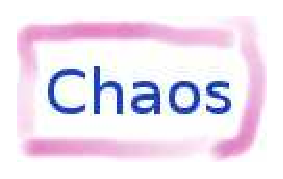
\includegraphics{TUDbeamer-logo}}
% \logo{\color{tudtextaccent}\large IFP}

\date{\today}

\begin{titleframe}
\end{titleframe}
\section{Background}
  \begin{frame}
  \frametitle{Outline}
  \begin{itemize}
  \setlength{\itemsep}{6pt}
  \item Background \& Motivation
  \item Related Work
  \item QuickDough Design Framework
  \item SCGRA Overlay Design \& Implementation
  \item FPGA Loop Accelerator Customization
  \item Experiments
  \begin{itemize}
    \setlength{\itemsep}{6pt}
    \item SCGRA Overlay Architecture
    \item Loop Accelerator Generation
    \item Loop Accelerator Customization
  \end{itemize}
  \item Conclusion
  \end{itemize}
  \end{frame}

  \begin{frame}
  \frametitle{Outline}
  \begin{itemize}
  \setlength{\itemsep}{6pt}
  \item \textbf{Background \& Motivation}
  \item Related Work
  \item QuickDough Design Framework
  \item SCGRA Overlay Design \& Implementation
  \item FPGA Loop Accelerator Customization
  \item Experiments
  \begin{itemize}
    \setlength{\itemsep}{6pt}
    \item SCGRA Overlay Architecture
    \item Loop Accelerator Generation
    \item Loop Accelerator Customization
  \end{itemize}
  \item Conclusion
  \end{itemize}
  \end{frame}

  \begin{frame}
  \frametitle{FPGA News}
  \begin{figure}
     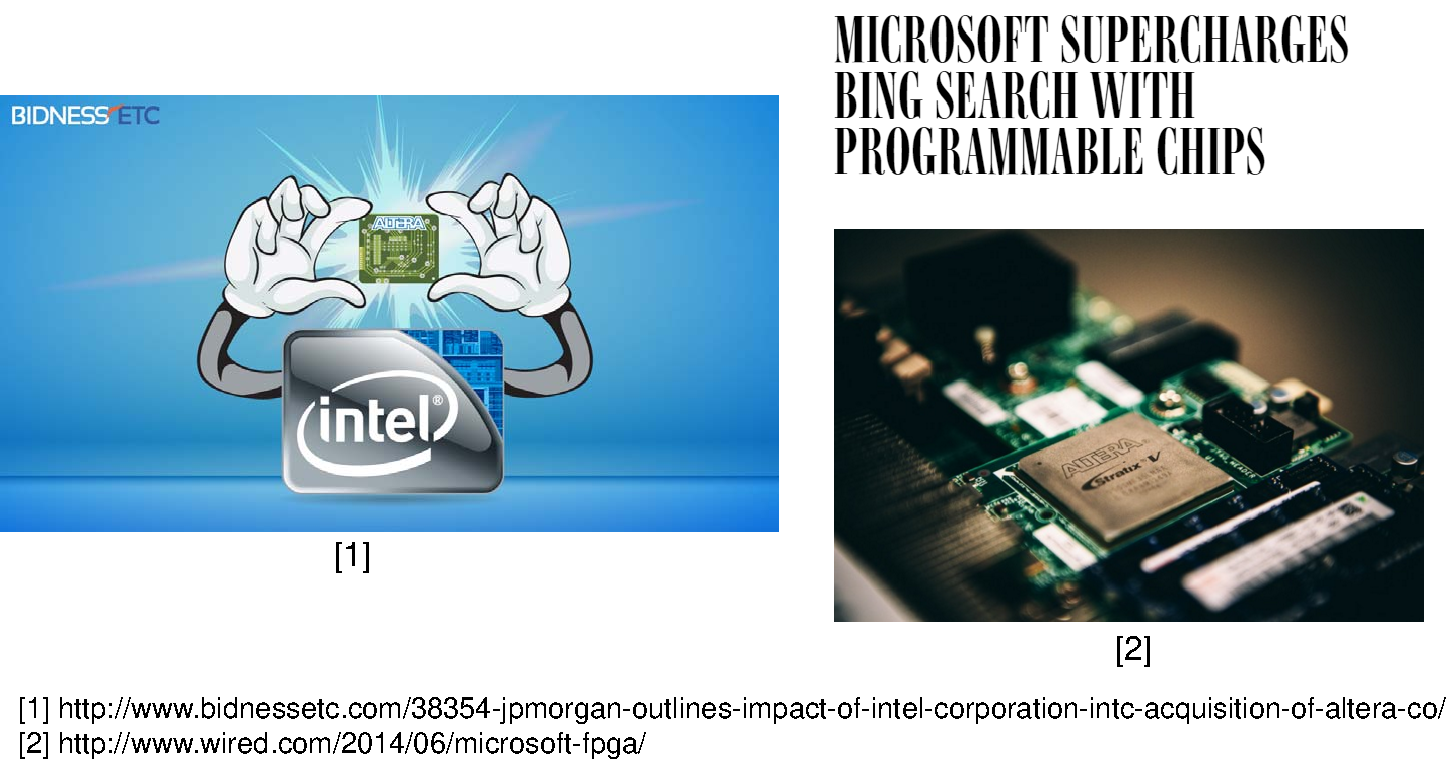
\includegraphics[width=.9\linewidth]{fpga-app2}
   \end{figure}

  \end{frame}
  \begin{frame}
  \frametitle{Advantages of Using FPGAs}
    \vspace{-0.6em}
    Successful demonstrations of using FPGA as hardware accelerators can be found in multitude of disciplines.
    \begin{figure}
      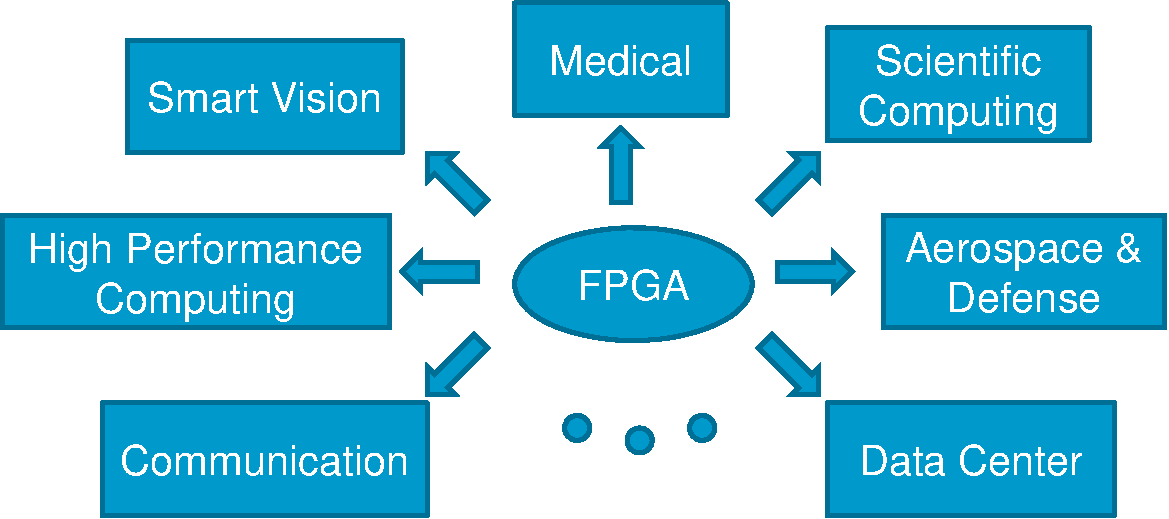
\includegraphics[width=.7\linewidth]{fpga-app}
    \end{figure}
		  
    General advantages of using FPGAs:
    \begin{itemize}
      \item \textbf{High energy efficiency}
      \item \textbf{Low latency, real-time processing}
      \item \textbf{Competitive performance}
      \item \textbf{...}
    \end{itemize}
  \end{frame}

  \begin{frame}
  \frametitle{Hybrid CPU-FPGA Computing System}
    \vspace{-0.7em}
    \begin{itemize}
    \item FPGA: deep pipelining, massive fine-grained parallelism, 
      fixed data flow graph, weird bit manipulation, low-latency 
      real-time processing, ...
    \item CPU: complex software environment such as OS, GUI, ...
    \end{itemize}
    \begin{figure}
      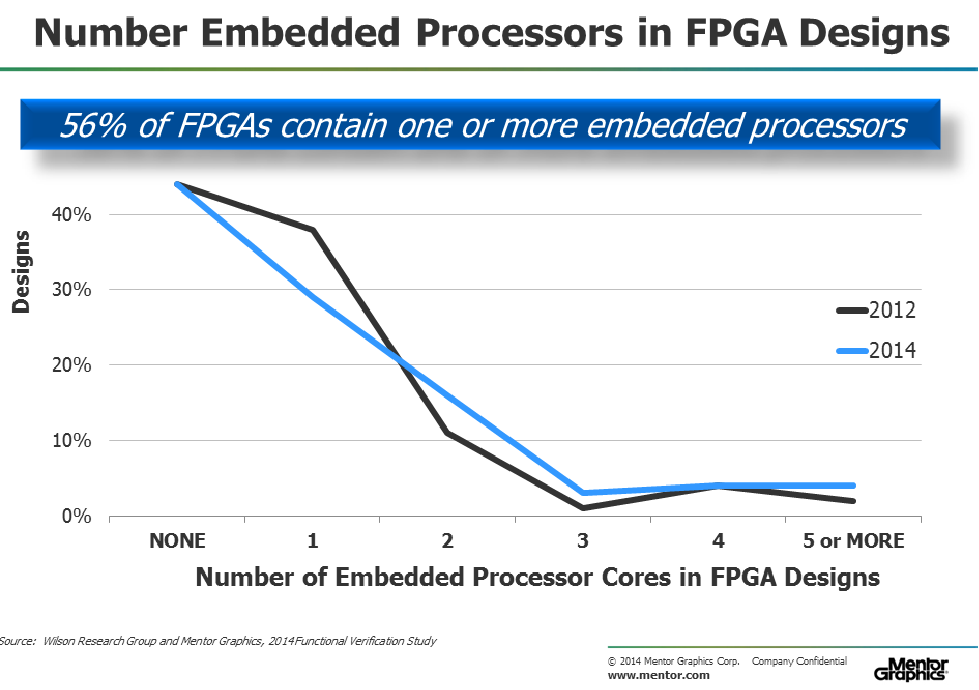
\includegraphics[width=.6\linewidth]{fpga-accelerator}
    \end{figure}
  \end{frame}

  \begin{frame}
  \frametitle{Challenges of Using FPGAs as Accelerators}
    \vspace{-1em}
    \begin{figure}
      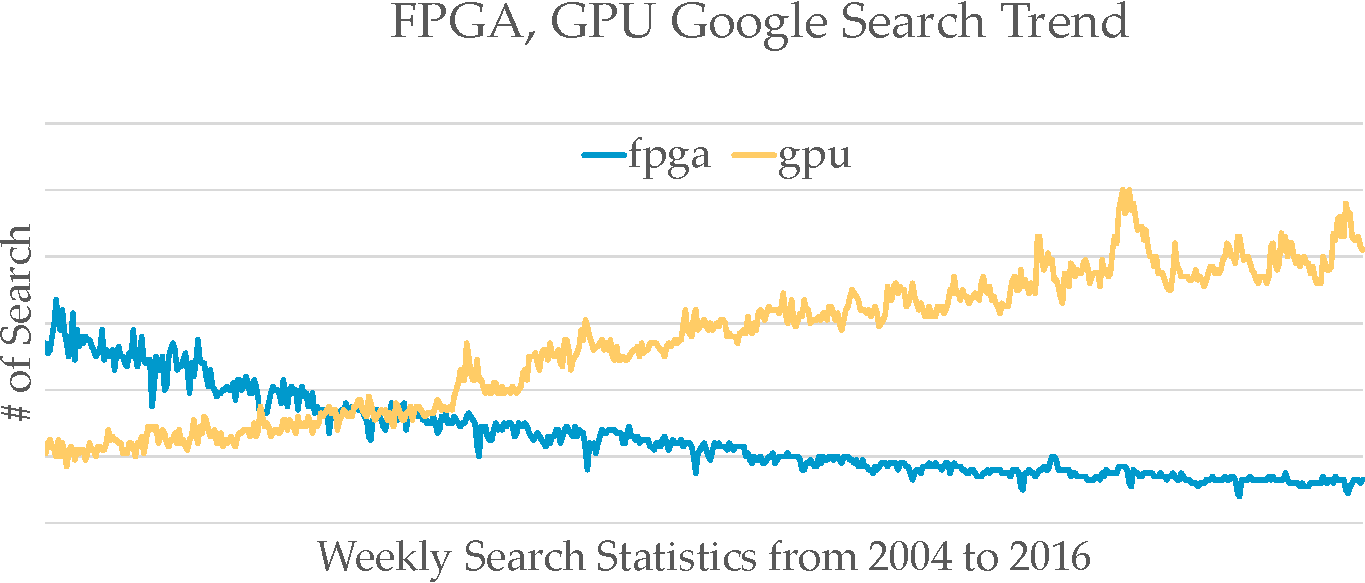
\includegraphics[width=.6\linewidth]{gpu-trend}
    \end{figure}
    \begin{figure}
      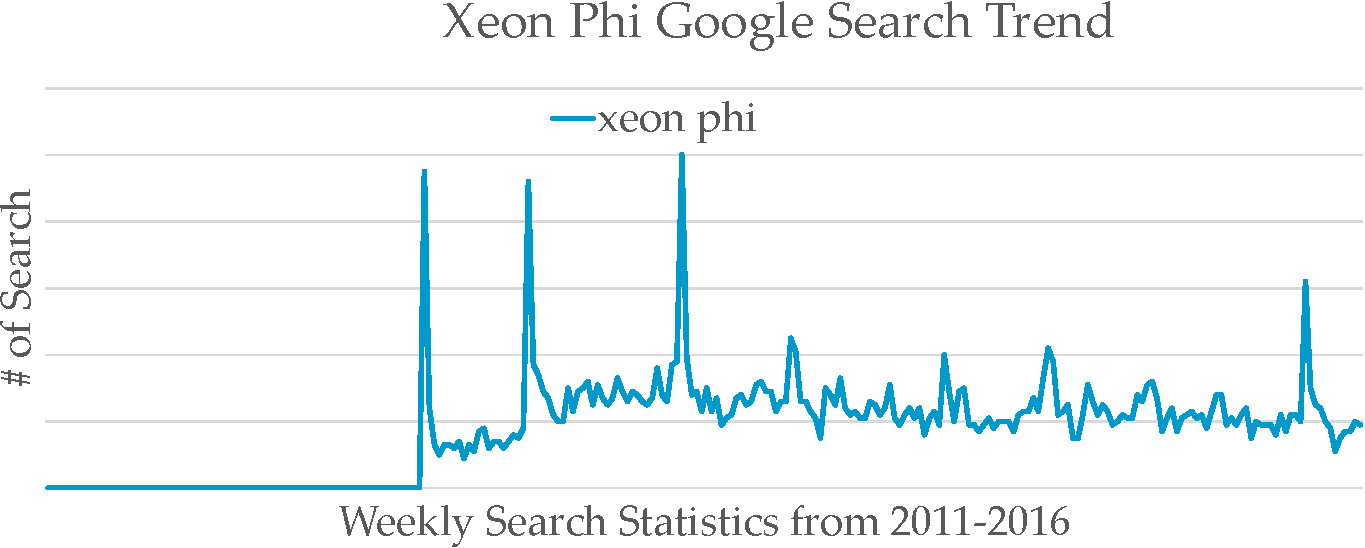
\includegraphics[width=.6\linewidth]{xeon-trend}
    \end{figure}
    \centering{
    \textbf{5/10} of the top10 super computer systems are using GPU or Xeon Phi as hardware accelerators while \textbf{none} of them using FPGAs as accelerators.}
  \end{frame}
   
   \begin{frame}
   \frametitle{Obstacles to the Adoption of FPGA Accelerators}
   \begin{figure}
      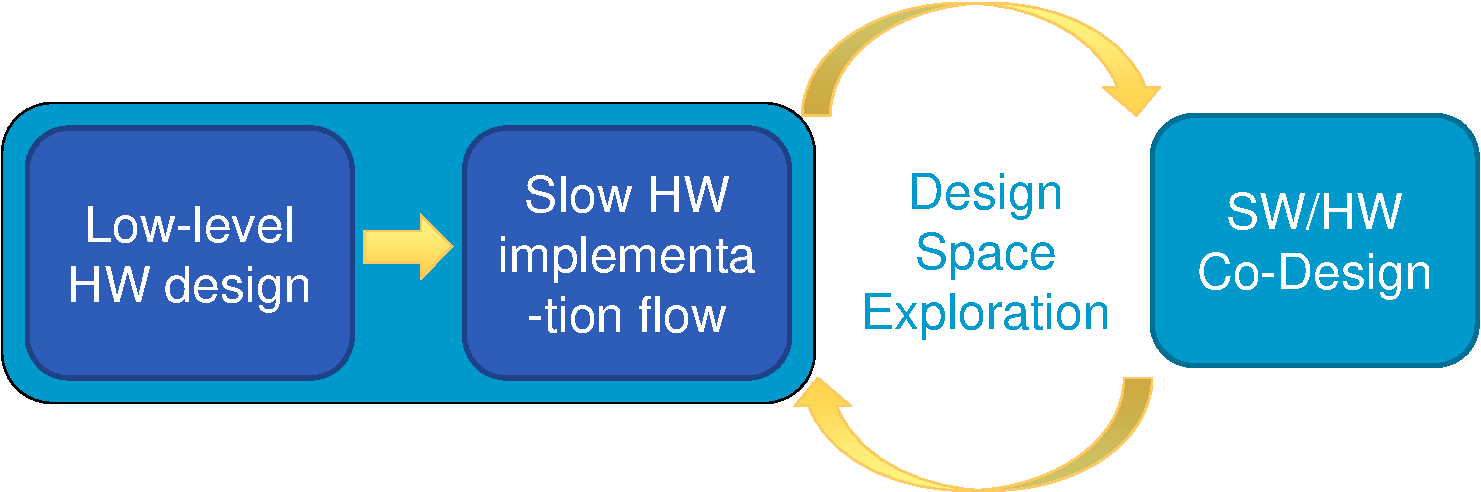
\includegraphics[width=.7\linewidth]{fpga-challenge-overview}
   \end{figure}

   Major obstacles --> Low design productivity:
   \begin{itemize}
   \item Low-level circuit design
   \item \textbf{Lengthy FPGA implementation}
   \item \textbf{Complex HW/SW co-design}
   \item \textbf{Challenging design space exploration}
   \item \textbf{...}
   \end{itemize}
   \end{frame}
   
\section{Related Work}
  \begin{frame}
  \frametitle{Outline}
  \begin{itemize}
  \setlength{\itemsep}{6pt}
  \item Background \& Motivation
  \item \textbf{Related Work}
  \item QuickDough Design Framework
  \item SCGRA Overlay Design \& Implementation
  \item FPGA Loop Accelerator Customization
  \item Experiments
  \begin{itemize}
    \setlength{\itemsep}{6pt}
    \item SCGRA Overlay Architecture
    \item Loop Accelerator Generation
    \item Loop Accelerator Customization
  \end{itemize}
  \item Conclusion
  \end{itemize}
  \end{frame}

   \begin{frame}
   \frametitle{Approaches to Improve the Design Productivity}
   The community have tried to approach this problem from various angles:
   \vspace{0.6em}
   \begin{itemize}
   \item \textbf{Raise the abstraction level (HLS tools, LegUp, Vivado HLS, ...)}
   \item Provide HW/SW run-time support (BORPH, ReconOS, ...)
   \item \textbf{Reduce the FPGA implementation time (partial reconfiguration, hard macro, implementation algorithms, ...)}
   \item Provide FPGA debugging facilities
   \item \textbf{Automatic design space exploration}
   \item \textbf{...}
   \end{itemize}

   \vspace{2em}
   {\color{red}{\textbf{FPGA design productivity is greatly improved, but remains much lower compared to software development.}}}
   \end{frame}

   \begin{frame}
   \frametitle{High Level Synthesis}
   \vspace{-0.9em}
   \begin{figure}
      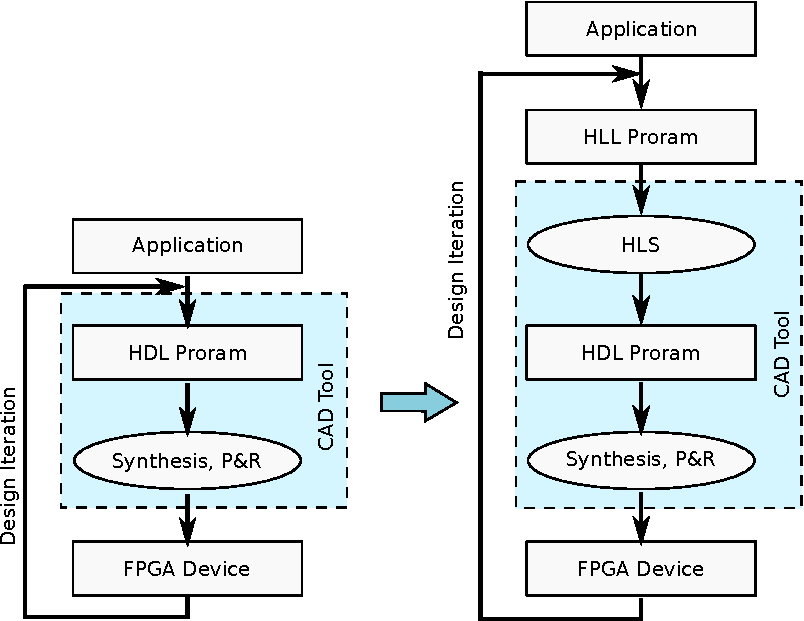
\includegraphics[width=.6\linewidth]{hls-compilation}
   \end{figure}
   \centering{
     \color{red}{\textbf{High level synthesis tools greatly improve the productivity of the designers.}}
   }
   \end{frame}

   \begin{frame}
   \frametitle{FPGA Accelerator Design Using HLS Tools}
   \begin{figure}
      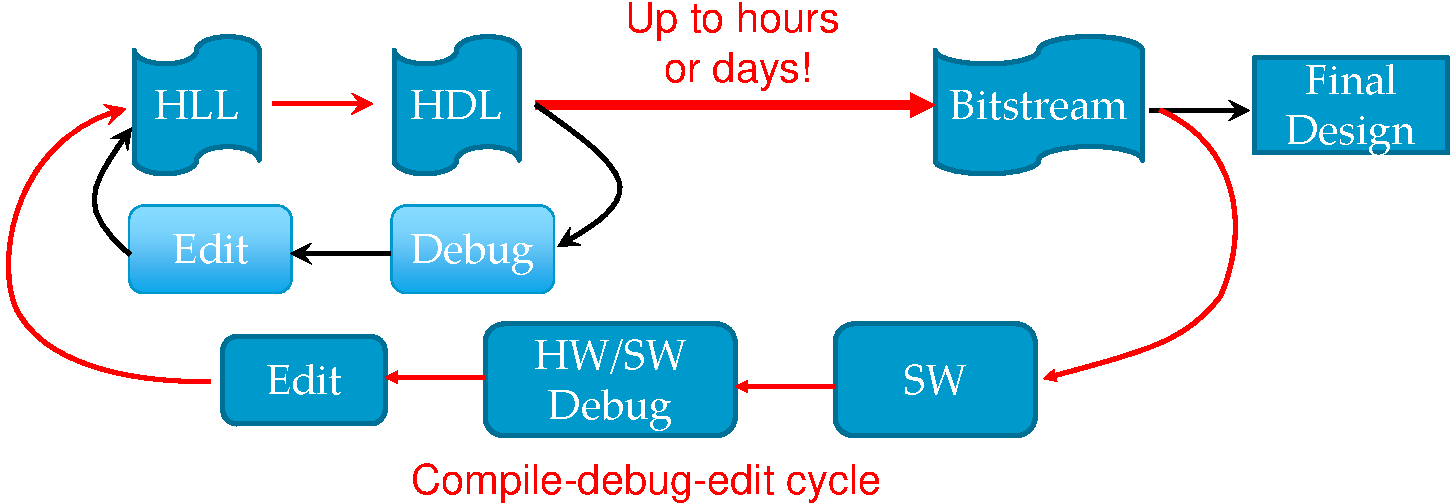
\includegraphics[width=.9\linewidth]{fpga-challenge-detail}
   \end{figure}

{\color{red}{\textbf{
Multiple levels of compile-debug-edit iterations are needed to develop a satisfying FPGA accelerator. The implementation process remains critical to the overall productivity.}}}
   \end{frame}

   % Slide-1
   \begin{frame}
   \frametitle{Overlay Architecture}
   A two-step HW/SW compilation approach:
   \begin{figure}
      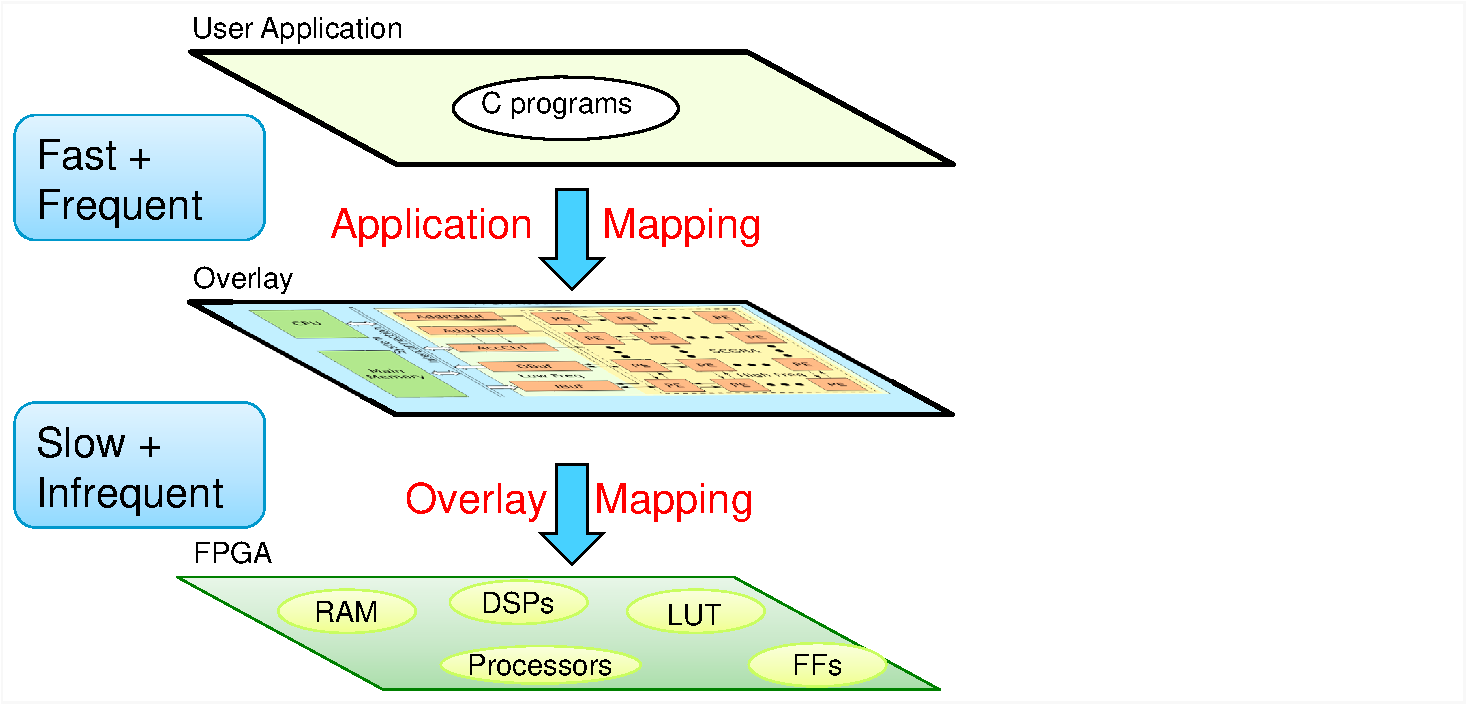
\includegraphics[width=.9\linewidth]{overlay-architecture1}
   \end{figure}
   \end{frame}

   % Slide-2
   \begin{frame}
   \frametitle{Overlay Architecture}
   A two-step HW/SW compilation approach:
   \begin{figure}
      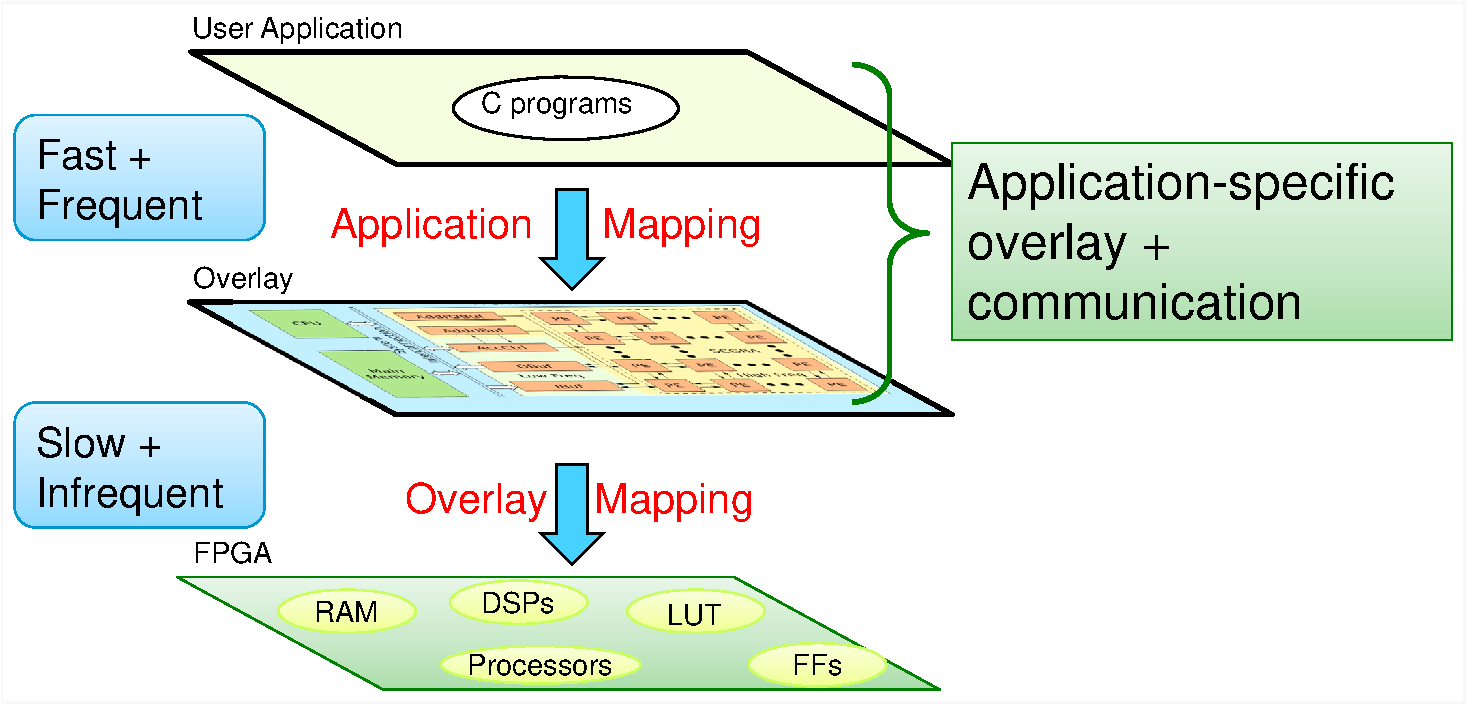
\includegraphics[width=.9\linewidth]{overlay-architecture2}
   \end{figure}
   \end{frame}
   
   \begin{frame}
   \frametitle{Classification of the Overlay Architectures}
   \vspace{-1em}
   \begin{figure}
      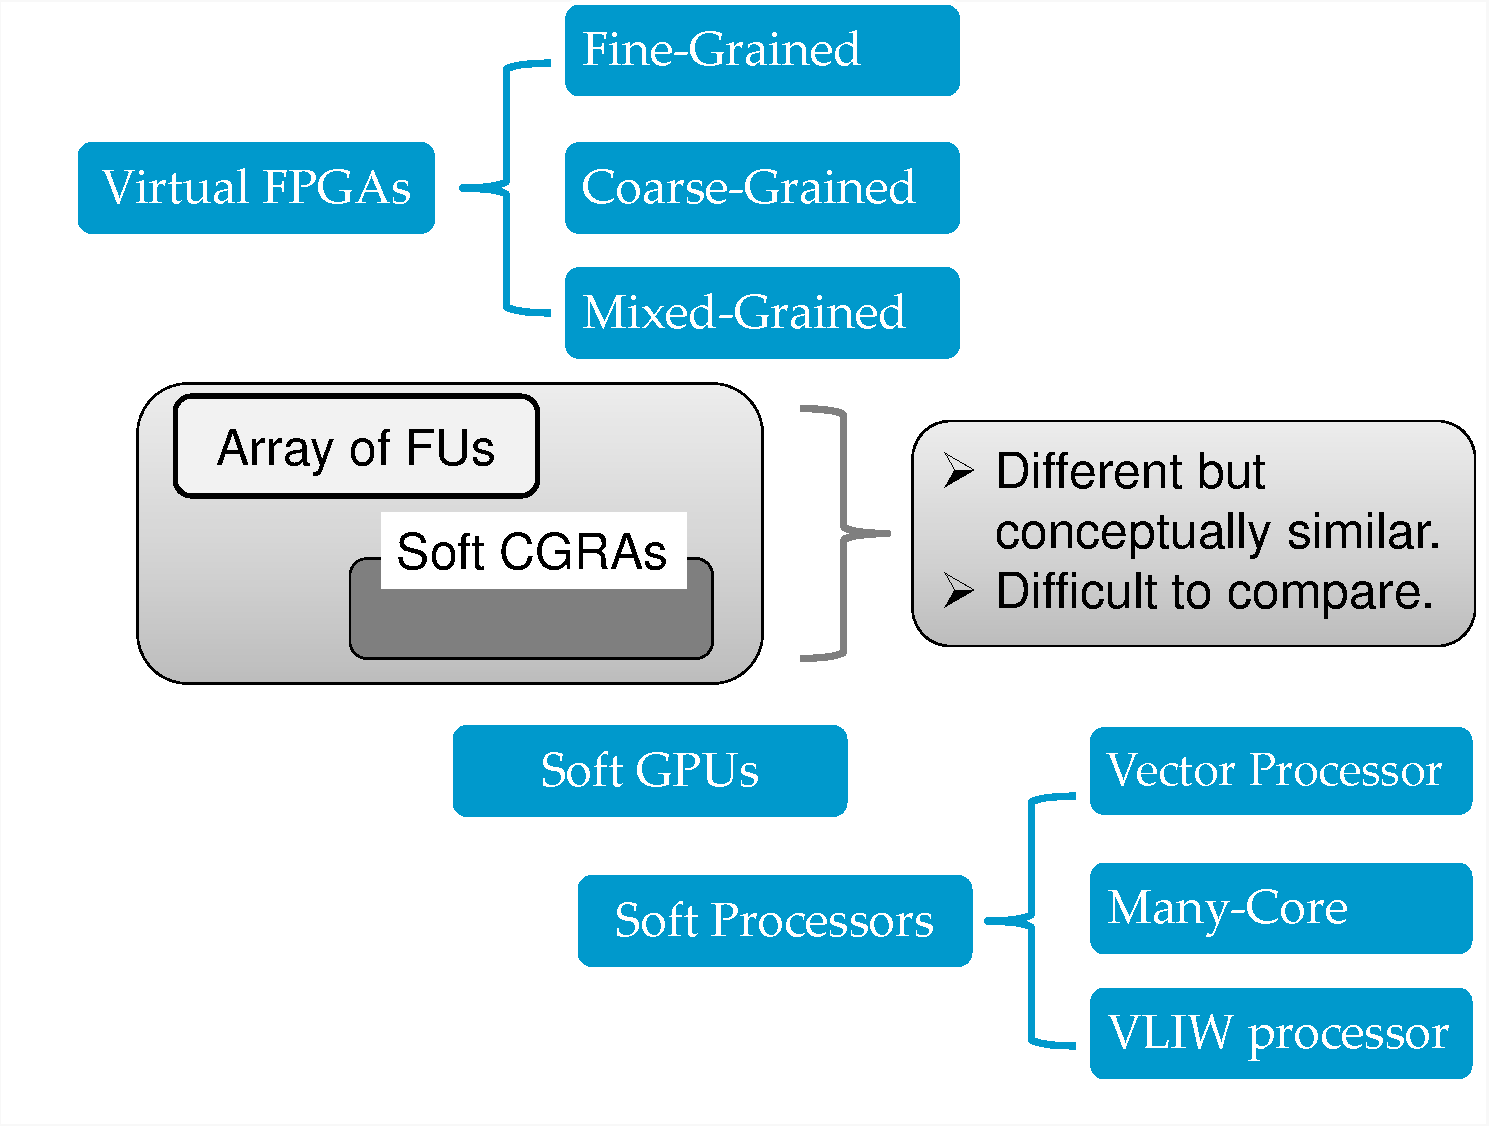
\includegraphics[width=.75\linewidth]{overlay-classification1}
   \end{figure}
   \end{frame}

   \begin{frame}
   \vspace{-1em}
   \frametitle{Classification of the Overlay Architectures}
   \begin{figure}
      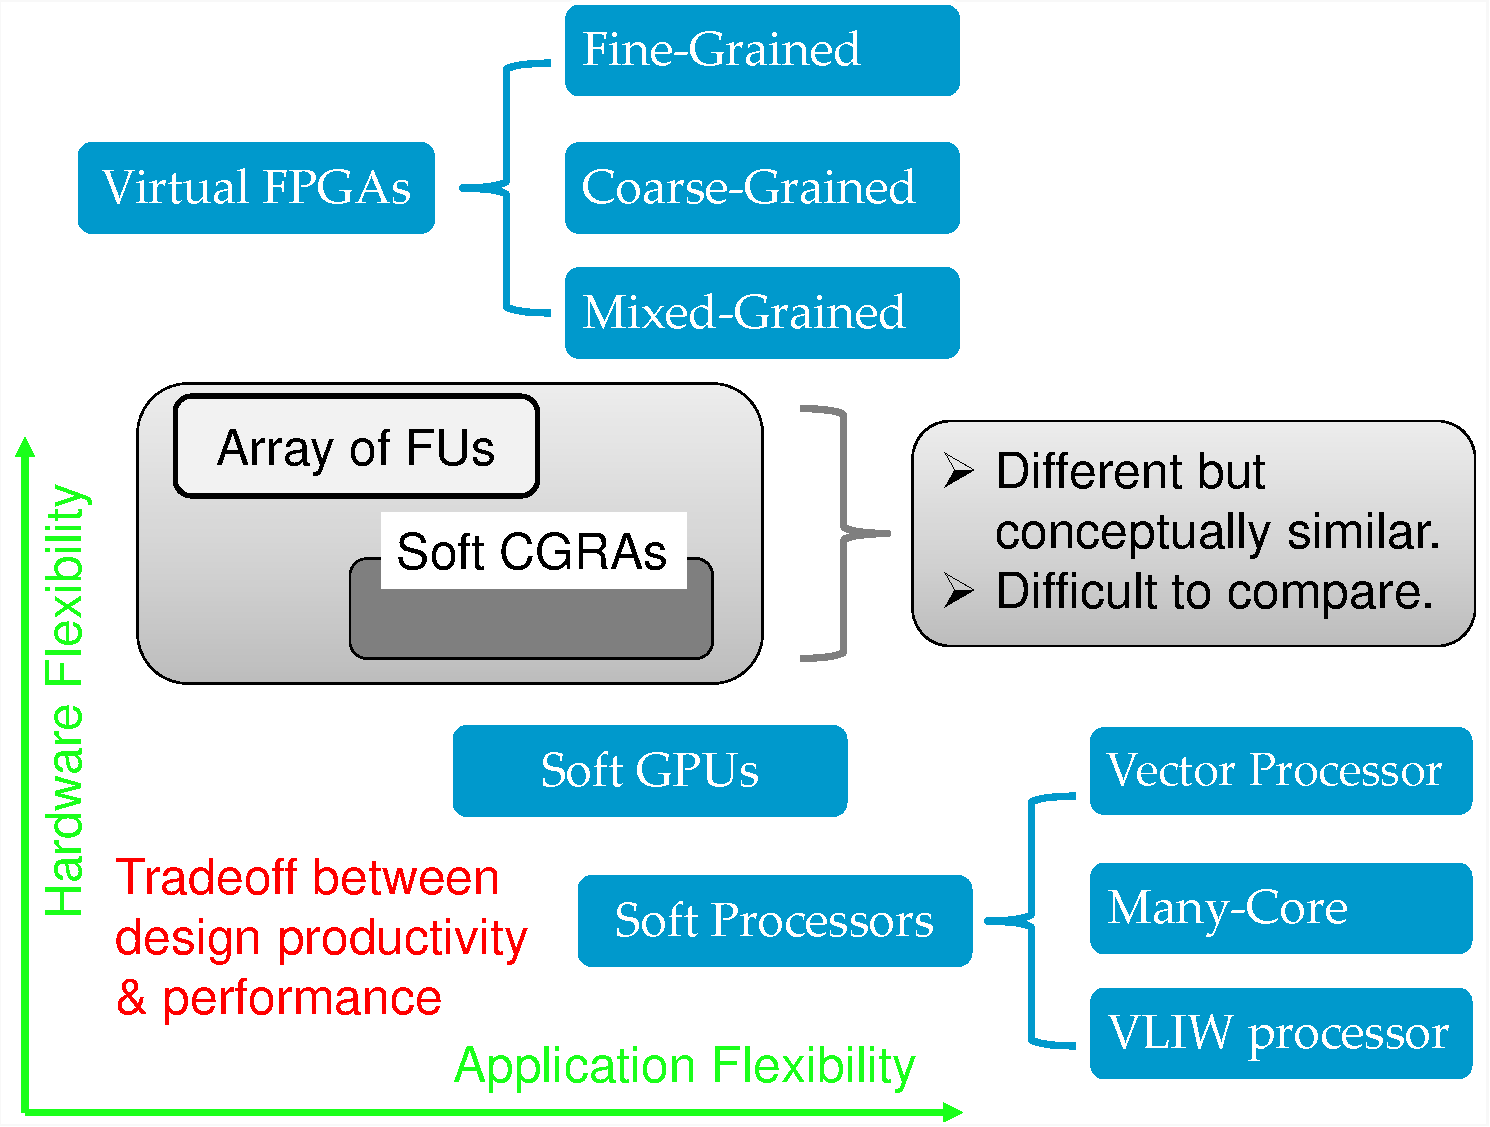
\includegraphics[width=.75\linewidth]{overlay-classification2}
   \end{figure}
   \end{frame}

   \begin{frame}
   \vspace{-1em}
   \frametitle{Classification of the Overlay Architectures}
   \begin{figure}
      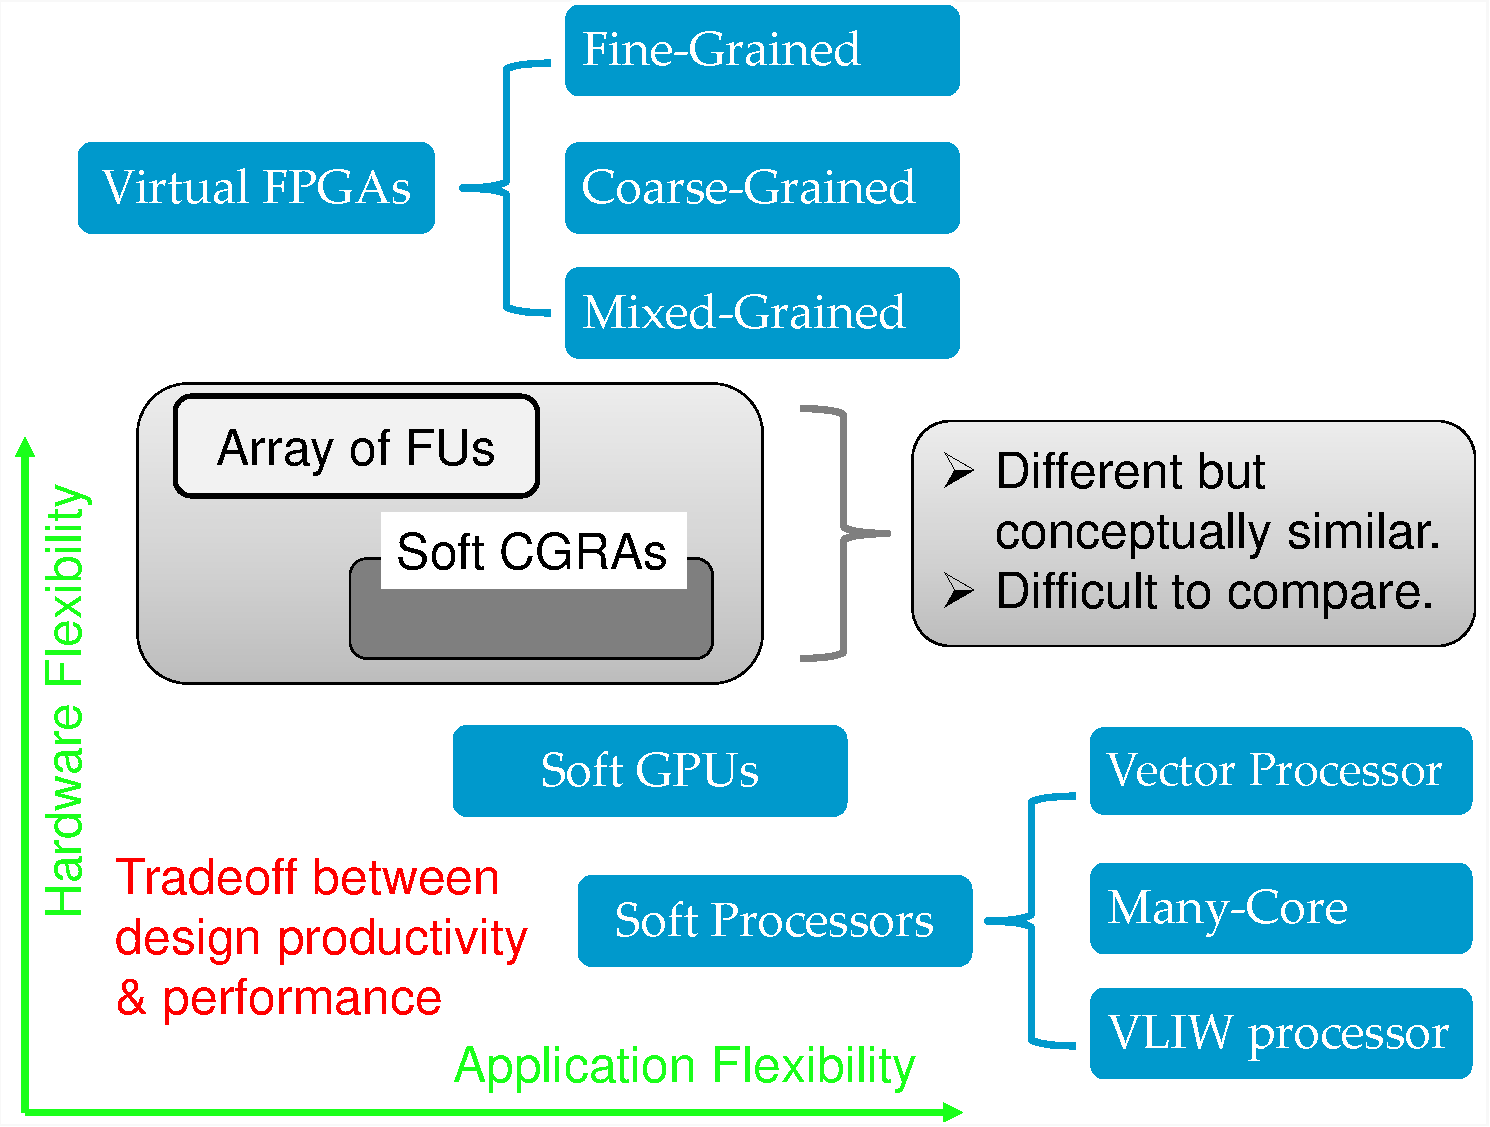
\includegraphics[width=.75\linewidth]{overlay-classification2}
   \end{figure}
   \vspace{-0.6em}
   \color{red}{It is difficult to quantify the 'complexity, compute intensity and even parallelism' of an application as well as design effort, so it is difficult to benchmark and compare.}
   \end{frame}

\section{QuickDough}
  \begin{frame}
  \frametitle{Outline}
  \begin{itemize}
  \setlength{\itemsep}{6pt}
  \item Background \& Motivation
  \item Related Work
  \item \textbf{QuickDough Design Framework}
  \item SCGRA Overlay Design \& Implementation
  \item FPGA Loop Accelerator Customization
  \item Experiments
  \begin{itemize}
    \setlength{\itemsep}{6pt}
    \item SCGRA Overlay Architecture
    \item Loop Accelerator Generation
    \item Loop Accelerator Customization
  \end{itemize}
  \item Conclusion
  \end{itemize}
  \end{frame}

  \begin{frame}
  \frametitle{QuickDough Overview}
  \vspace{-0.6em}
  A high productivity compilation framework for high-level applications on CPU-FPGA computers.
  \begin{itemize}
    \item Compiles software and FPGA accelerator design within the same framework
    \item Overall SW-like compile speed
  \end{itemize}

  \begin{figure}
     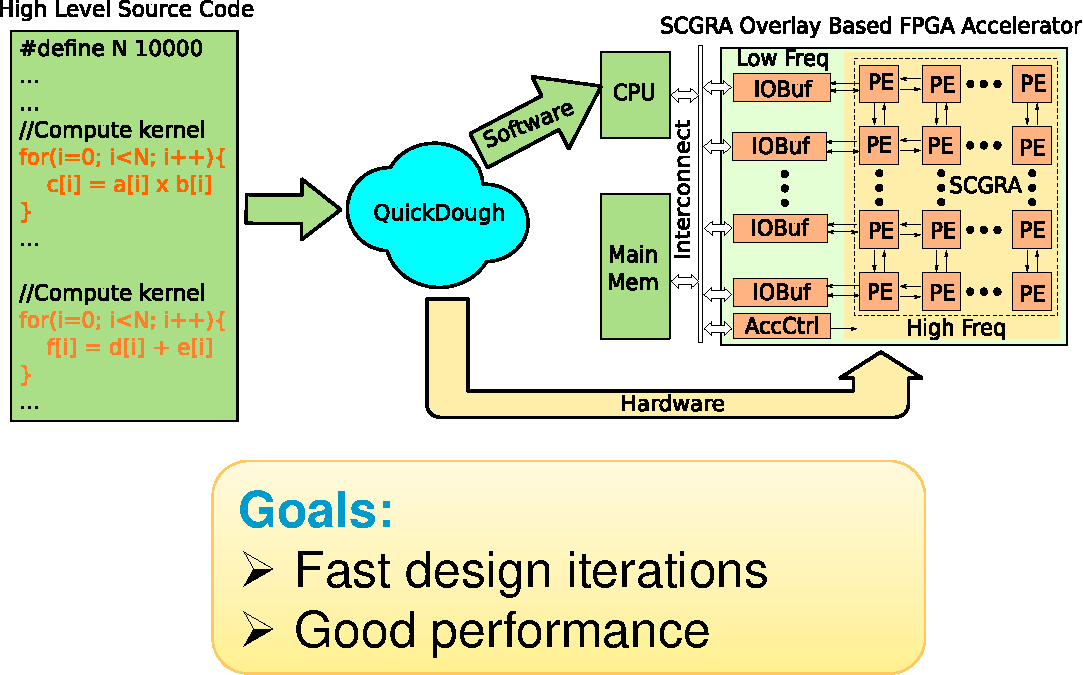
\includegraphics[width=.75\linewidth]{qd-overview}
  \end{figure}
  \end{frame}

  \begin{frame}
  \frametitle{QuickDough Design Flow}
  \begin{figure}
     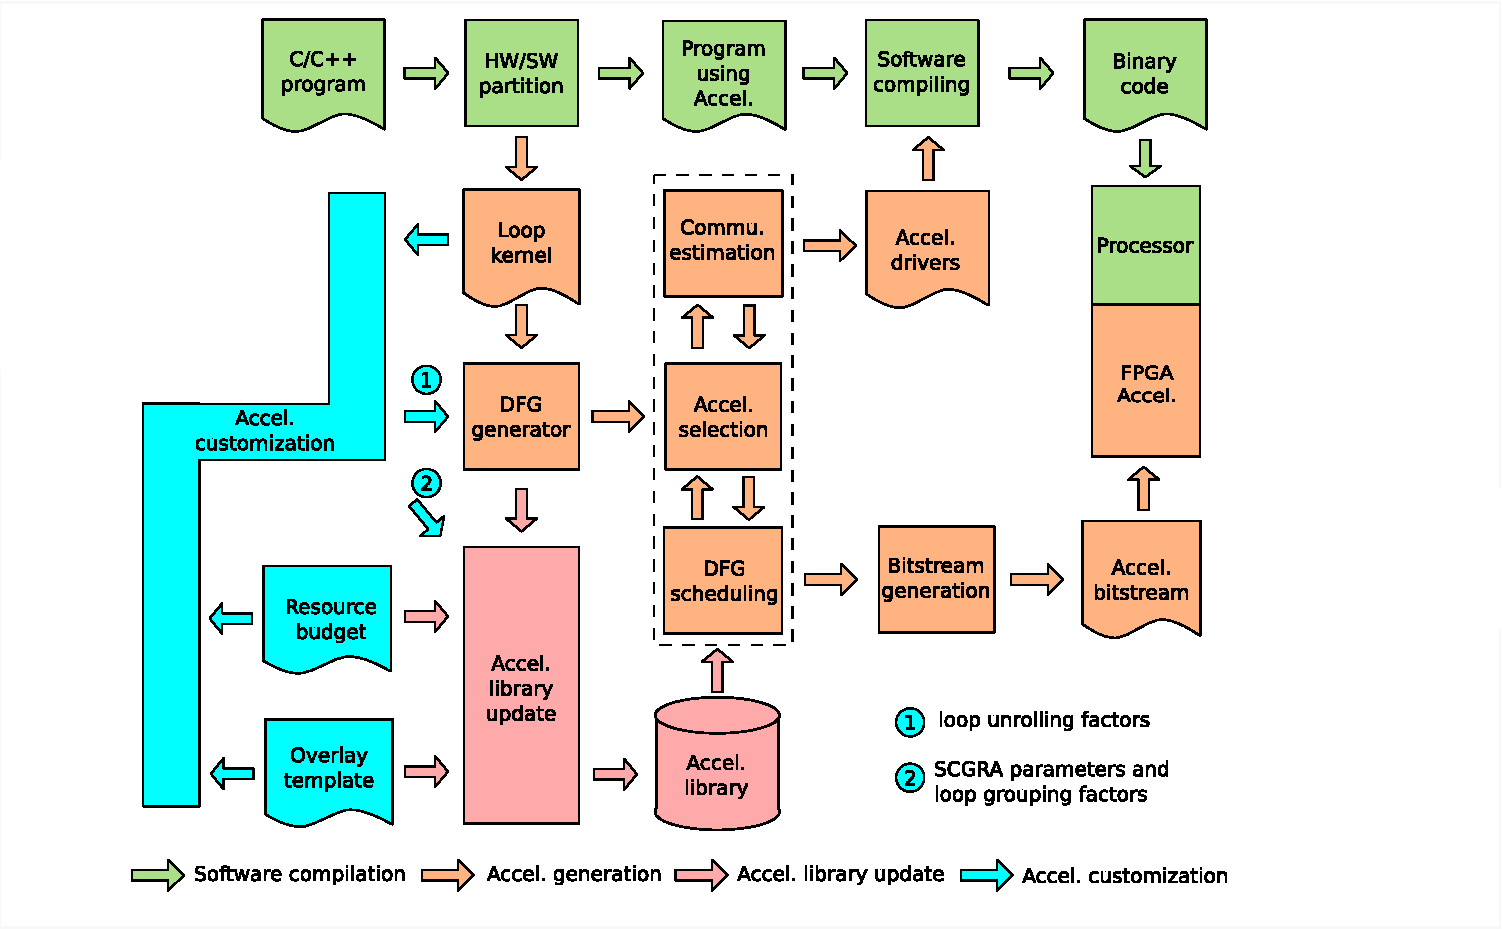
\includegraphics[width=.95\linewidth]{qd-flow1}
  \end{figure}
  \end{frame}

\begin{frame}
  \frametitle{QuickDough Design Flow}
  \begin{figure}
     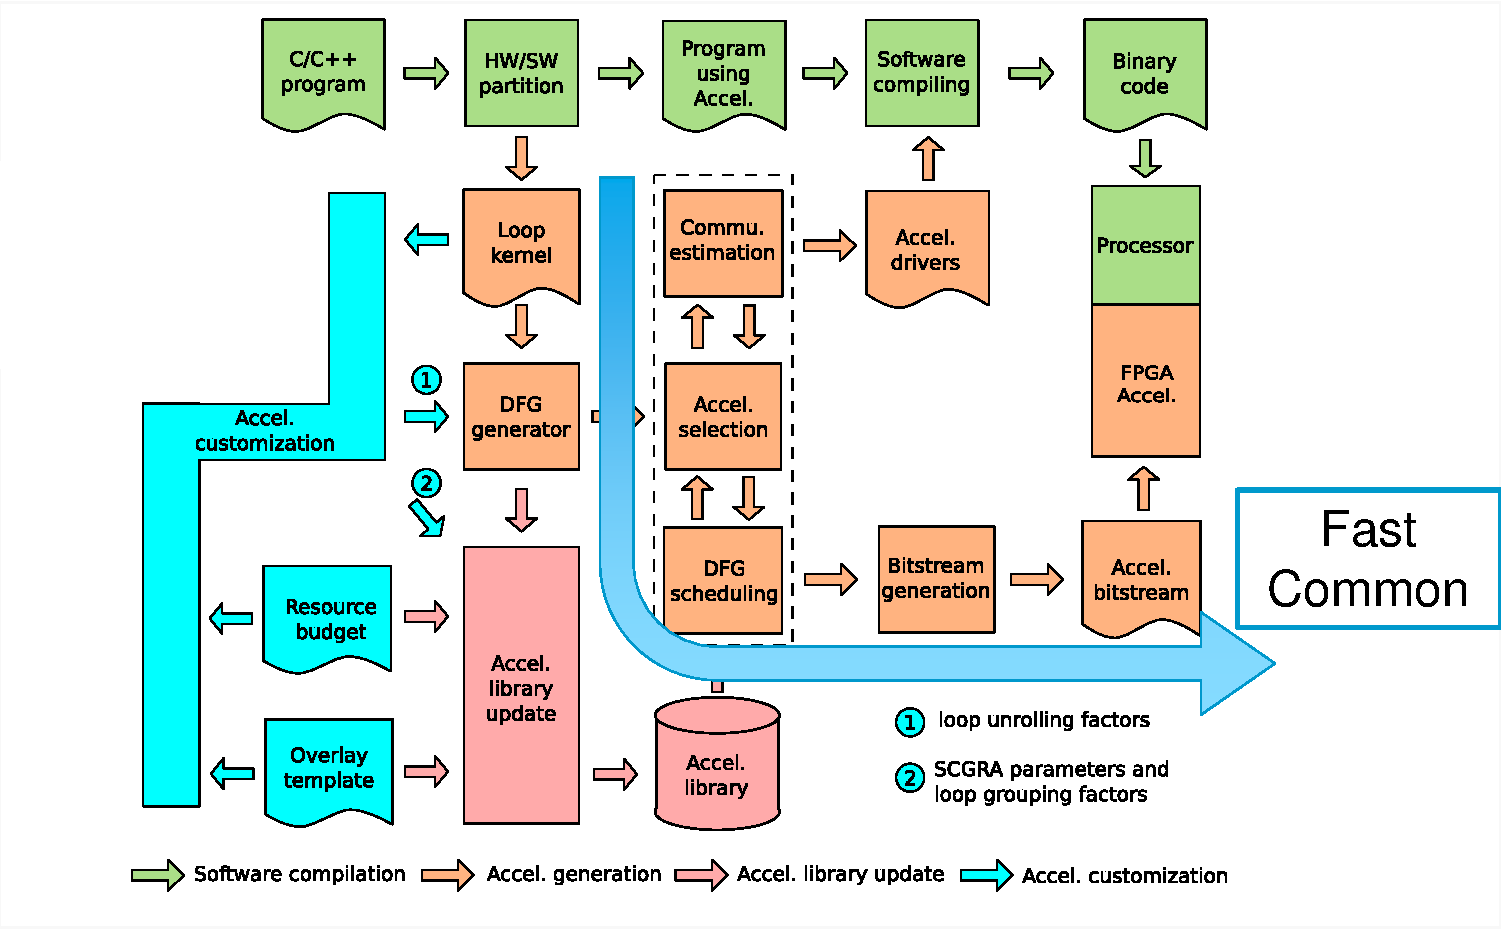
\includegraphics[width=.95\linewidth]{qd-flow2}
  \end{figure}
  \end{frame}

\begin{frame}
  \frametitle{Detailed Fast Common Route}
  \begin{figure}
     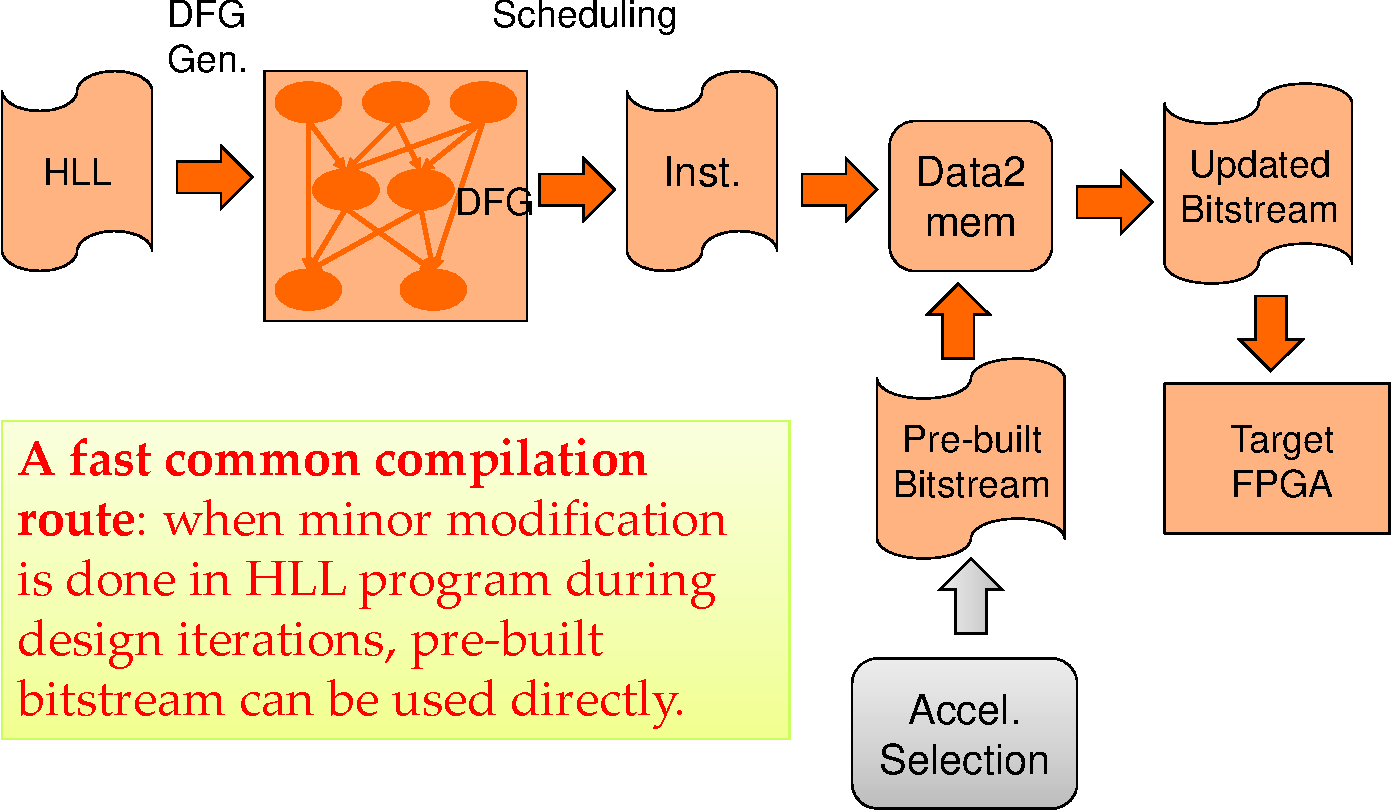
\includegraphics[width=.85\linewidth]{detailed-fast-route}
  \end{figure}
\end{frame}

\begin{frame}
  \frametitle{QuickDough Design Flow}
  \begin{figure}
     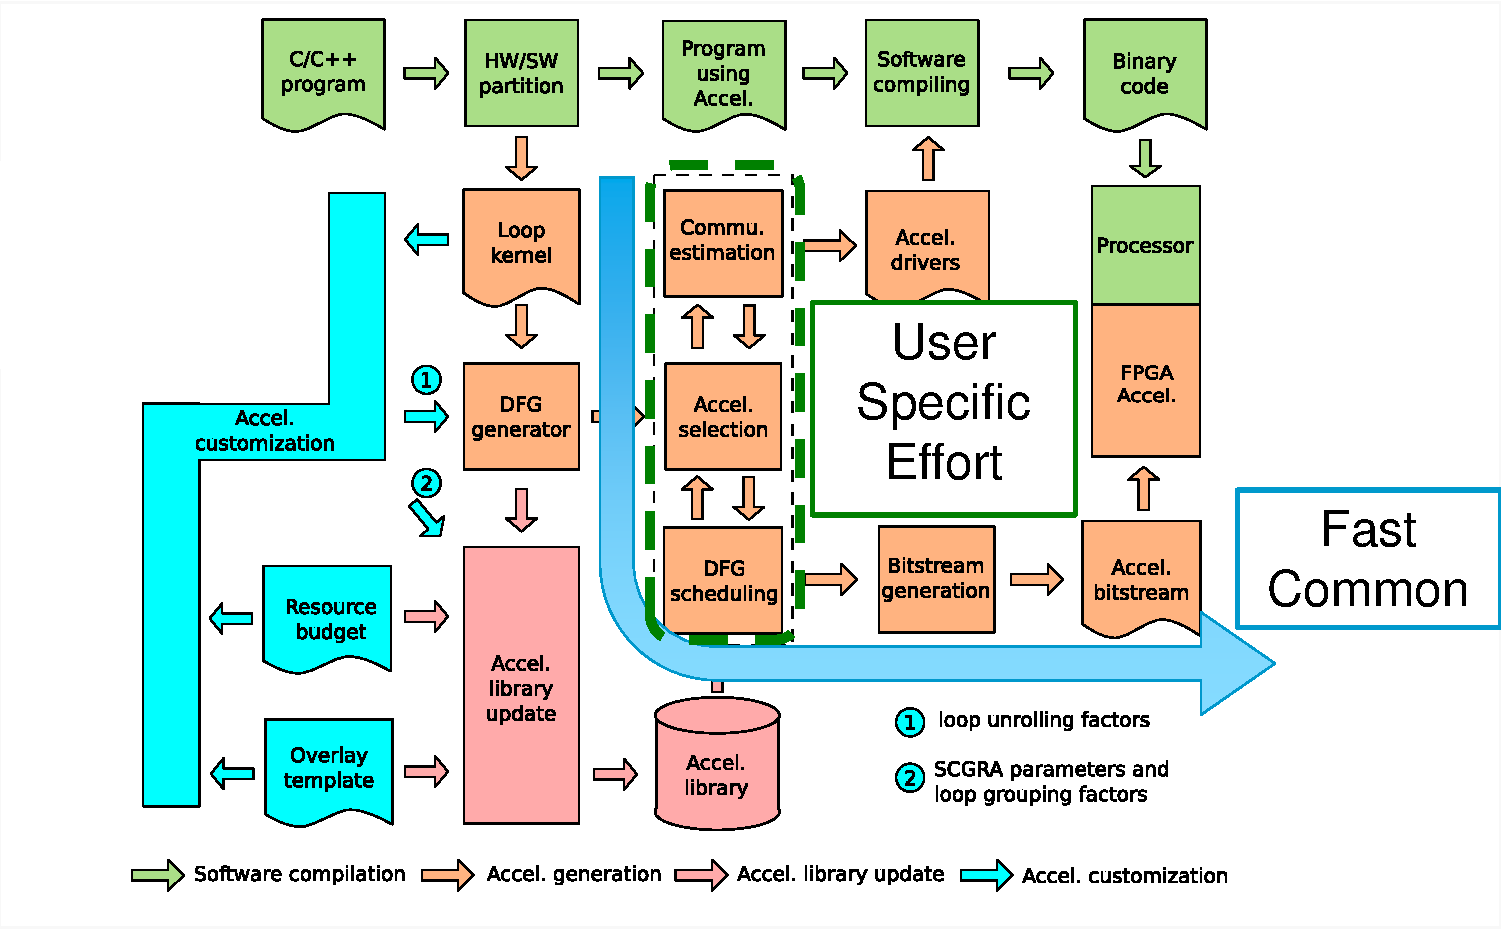
\includegraphics[width=.95\linewidth]{qd-flow3}
  \end{figure}
  \end{frame}


\begin{frame}
\frametitle{Accelerator Selection}
\vspace{-0.8em}
The accelerator library can be organized, so that the time consuming operation scheduling process can be reused to evaluate a group of configurations in the library. 

  \begin{figure}
     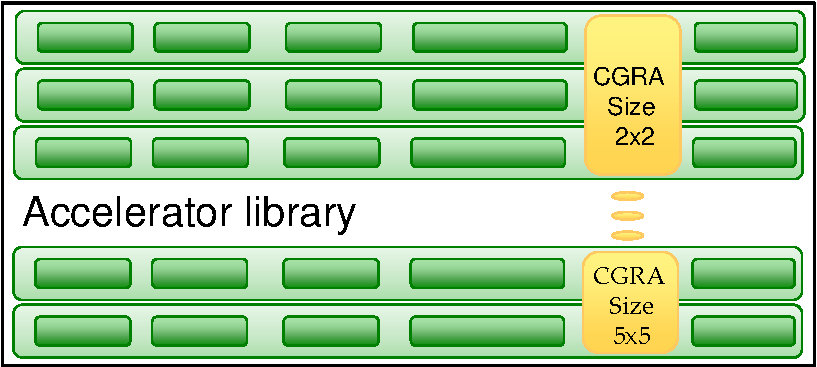
\includegraphics[width=.65\linewidth]{accel-sel3}
  \end{figure}
User specified accelerator selection strategy:
\begin{itemize}
   \item -O1 select the accelerator with smallest SCGRA size
   \item -O2 target three groups of accelerators with different SCGRA size (small, medium, large)
   \item -O3 full search
\end{itemize}
\end{frame}

\begin{frame}
  \frametitle{QuickDough Design Flow}
  \begin{figure}
     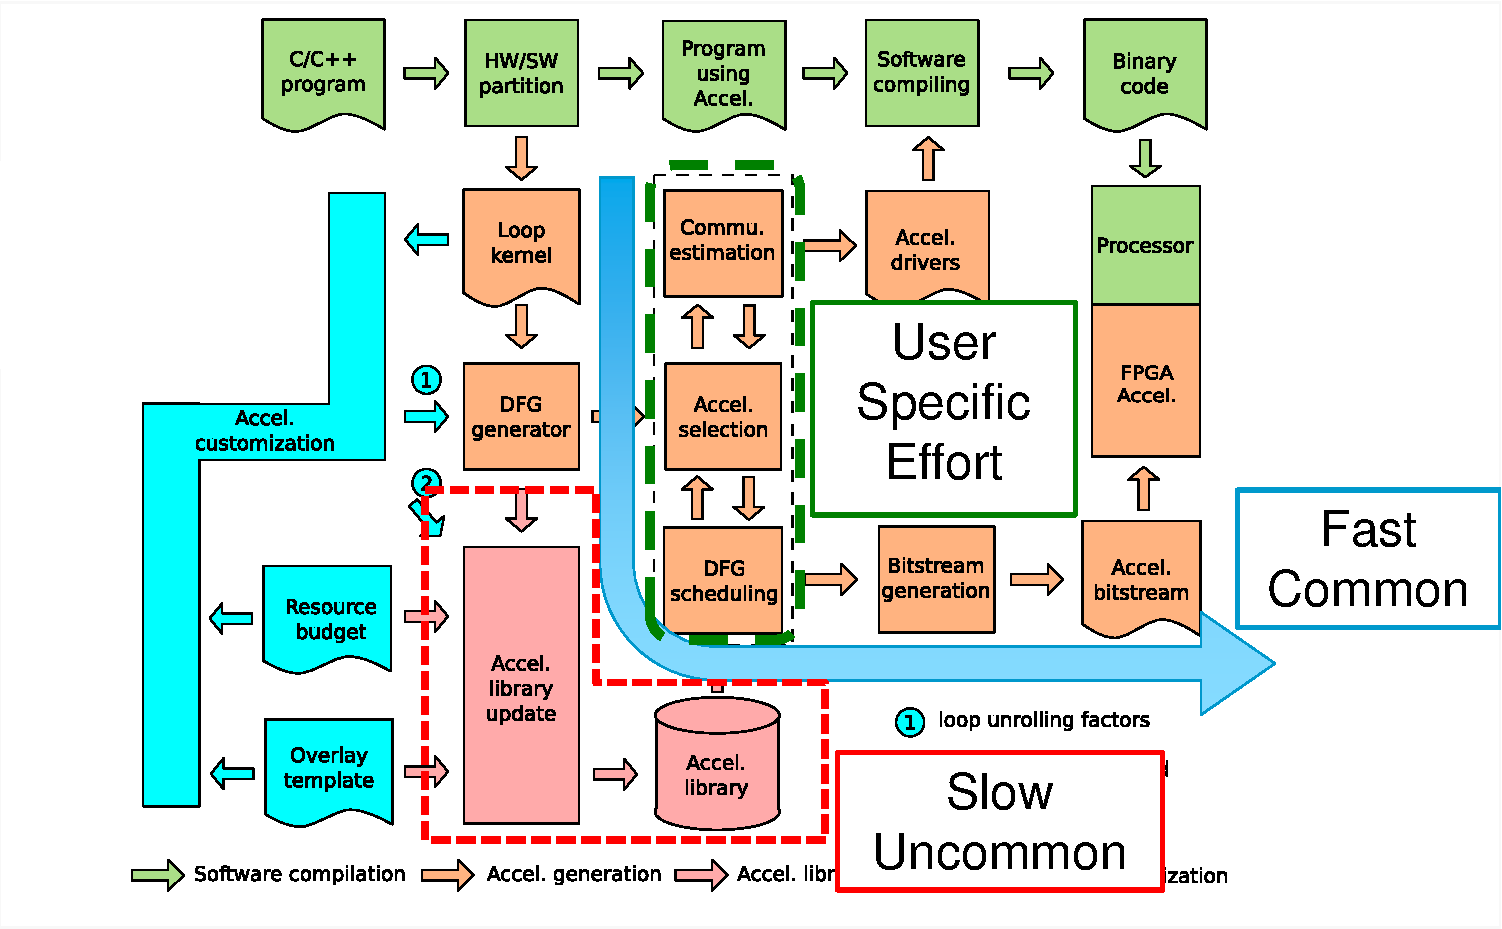
\includegraphics[width=.95\linewidth]{qd-flow4}
  \end{figure}
\end{frame}

\begin{frame}
\frametitle{Accelerator Library Pre-build \& Update}
  \begin{figure}
     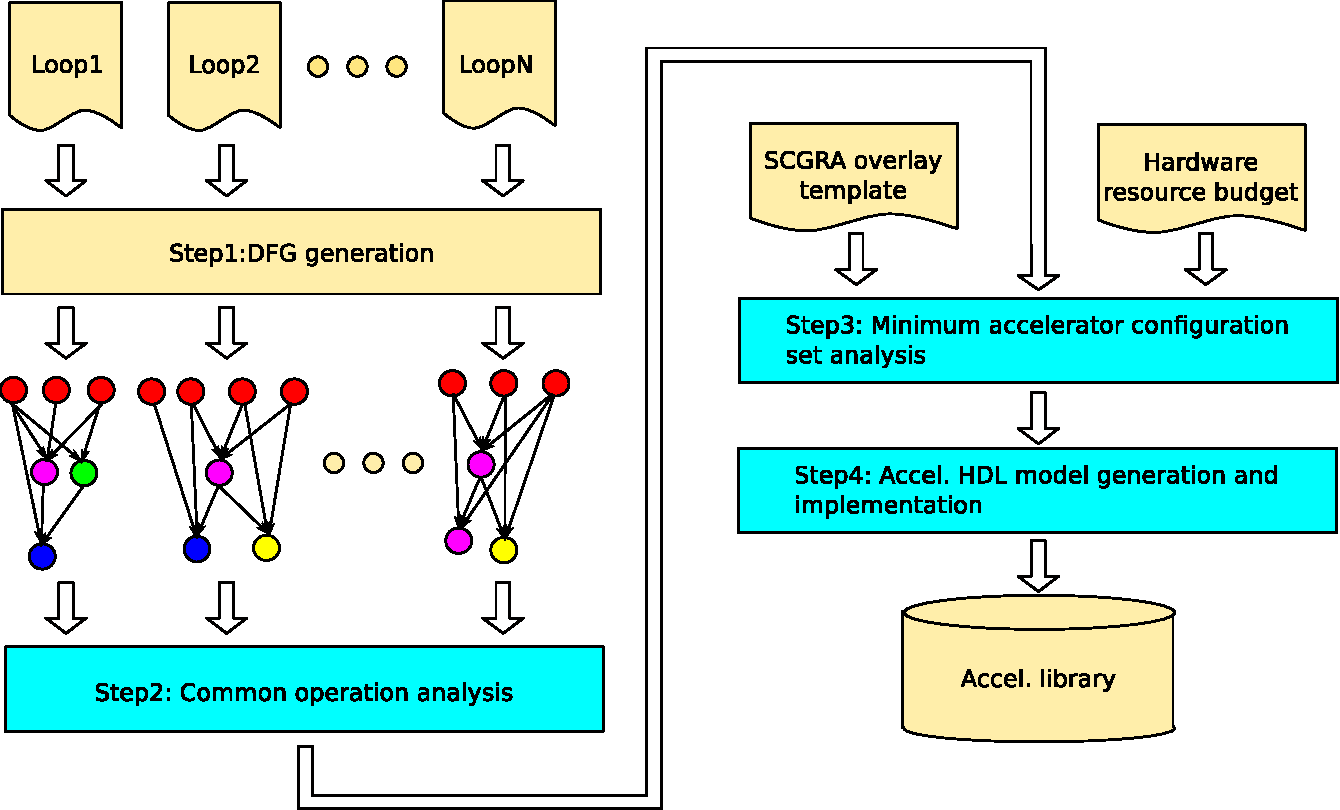
\includegraphics[width=.85\linewidth]{lib-build}
  \end{figure}
\end{frame}

\begin{frame}
  \frametitle{QuickDough Design Flow}
  \begin{figure}
     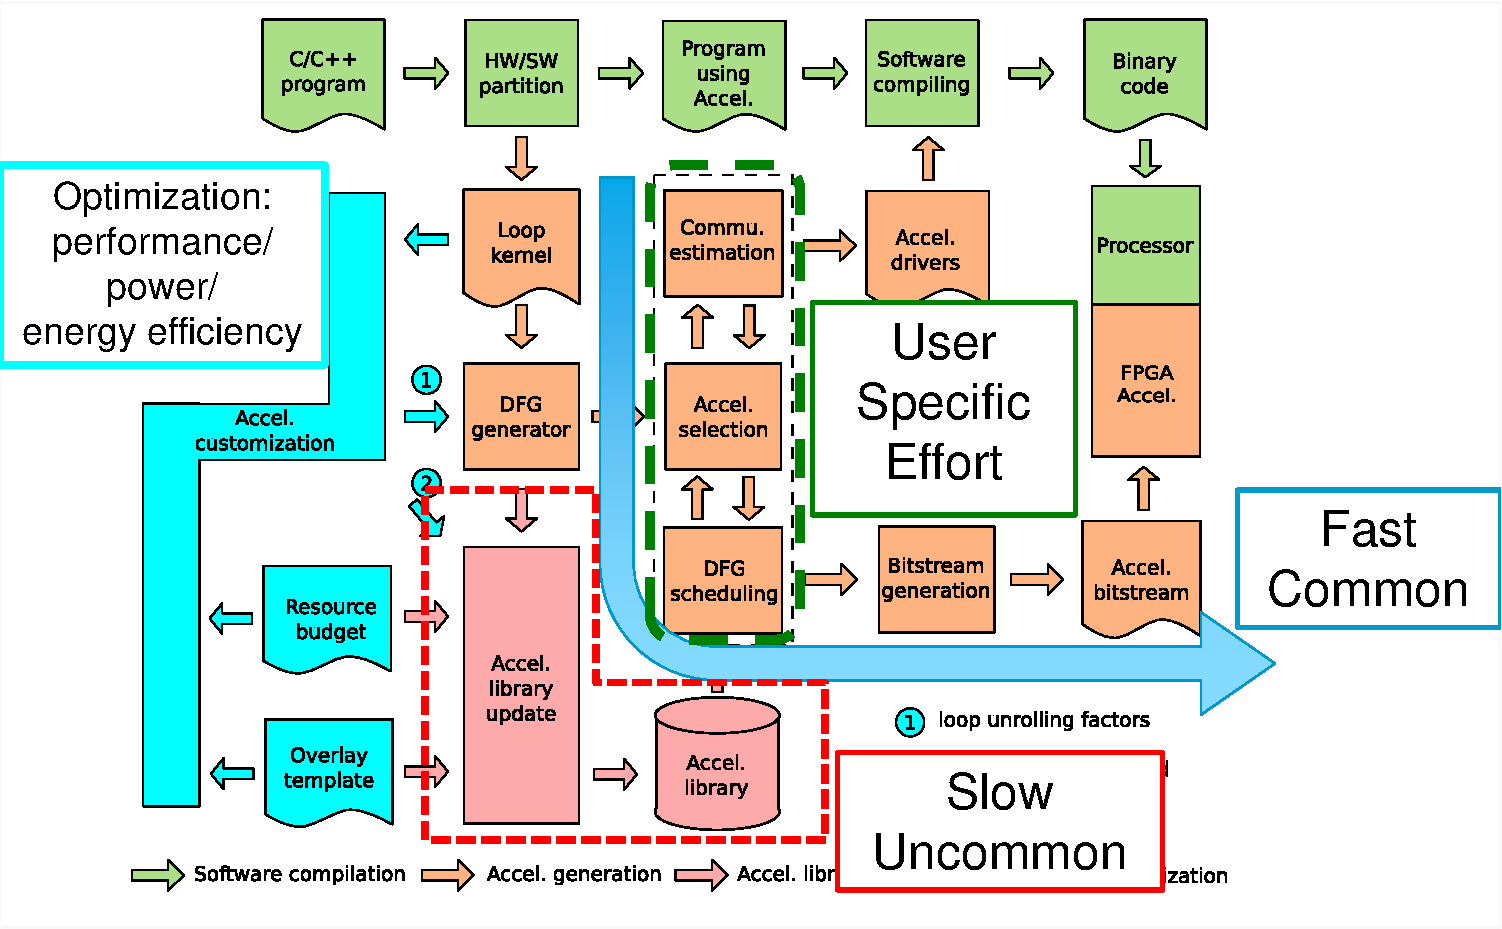
\includegraphics[width=.95\linewidth]{qd-flow5}
  \end{figure}
  \end{frame}

\section{CGRA Overlay}
  \begin{frame}
  \frametitle{Outline}
  \begin{itemize}
  \setlength{\itemsep}{6pt}
  \item Background \& Motivation
  \item Related Work
  \item QuickDough Design Framework
  \item \textbf{SCGRA Overlay Design \& Implementation}
  \item FPGA Loop Accelerator Customization
  \item Experiments
  \begin{itemize}
    \setlength{\itemsep}{6pt}
    \item SCGRA Overlay Architecture
    \item Loop Accelerator Generation
    \item Loop Accelerator Customization
  \end{itemize}
  \item Conclusion
  \end{itemize}
  \end{frame}

  \begin{frame}
  \frametitle{Proposed Soft CGRA Overlay}
  Design principles:
  \begin{itemize}
  \item Highly pipelined --> performance acceleration
  \item Reconfigurable --> Application-specific optimization
  \item Simple and easy to extend
  \item Make best use of the underlying FPGA resources
  \end{itemize}

  \begin{figure}
     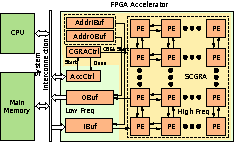
\includegraphics[width=.6\linewidth]{scgra-accelerator}
  \end{figure}
  \end{frame}

  \begin{frame}
  \frametitle{Processing Element (PE)}
  \vspace{1em}
  \begin{figure}
     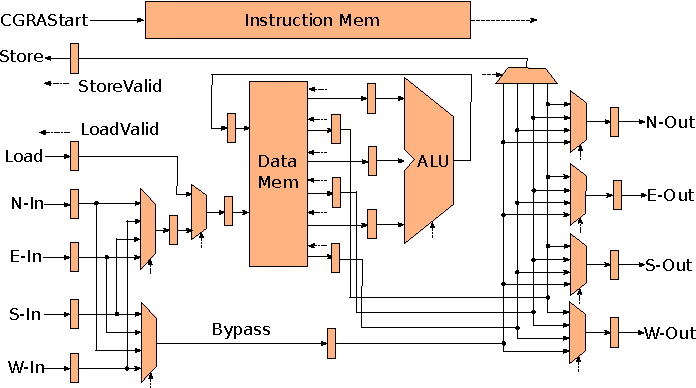
\includegraphics[width=.75\linewidth]{pe}
  \end{figure}
 When there are sufficient parallel operations in the data memory, the PE can perform 1 operation per cycle ideally while bypassing one data to the neighboring PE at the same time.
  \end{frame}

  \begin{frame}
  \frametitle{ALU}
  \vspace{-1em}
  \begin{figure}
    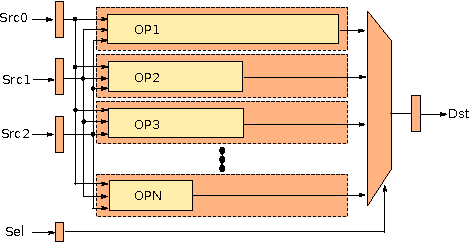
\includegraphics[width=.55\linewidth]{alu}
  \end{figure}
  \vspace{-0.5em}
  \begin{figure}
    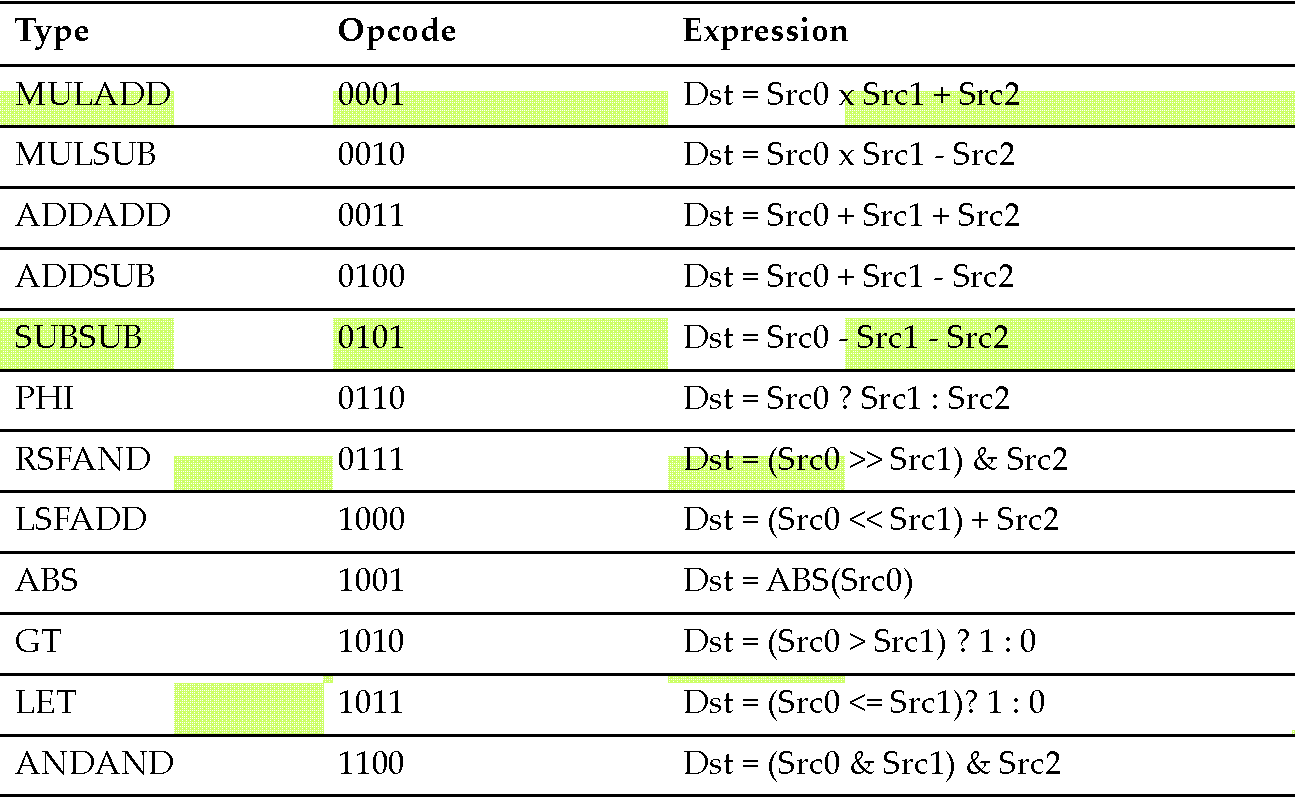
\includegraphics[width=.55\linewidth]{op-table}
  \end{figure}
  \end{frame}

  \begin{frame}
  \frametitle{Accelerator Controller and CGRA Controller}
  \begin{figure}
    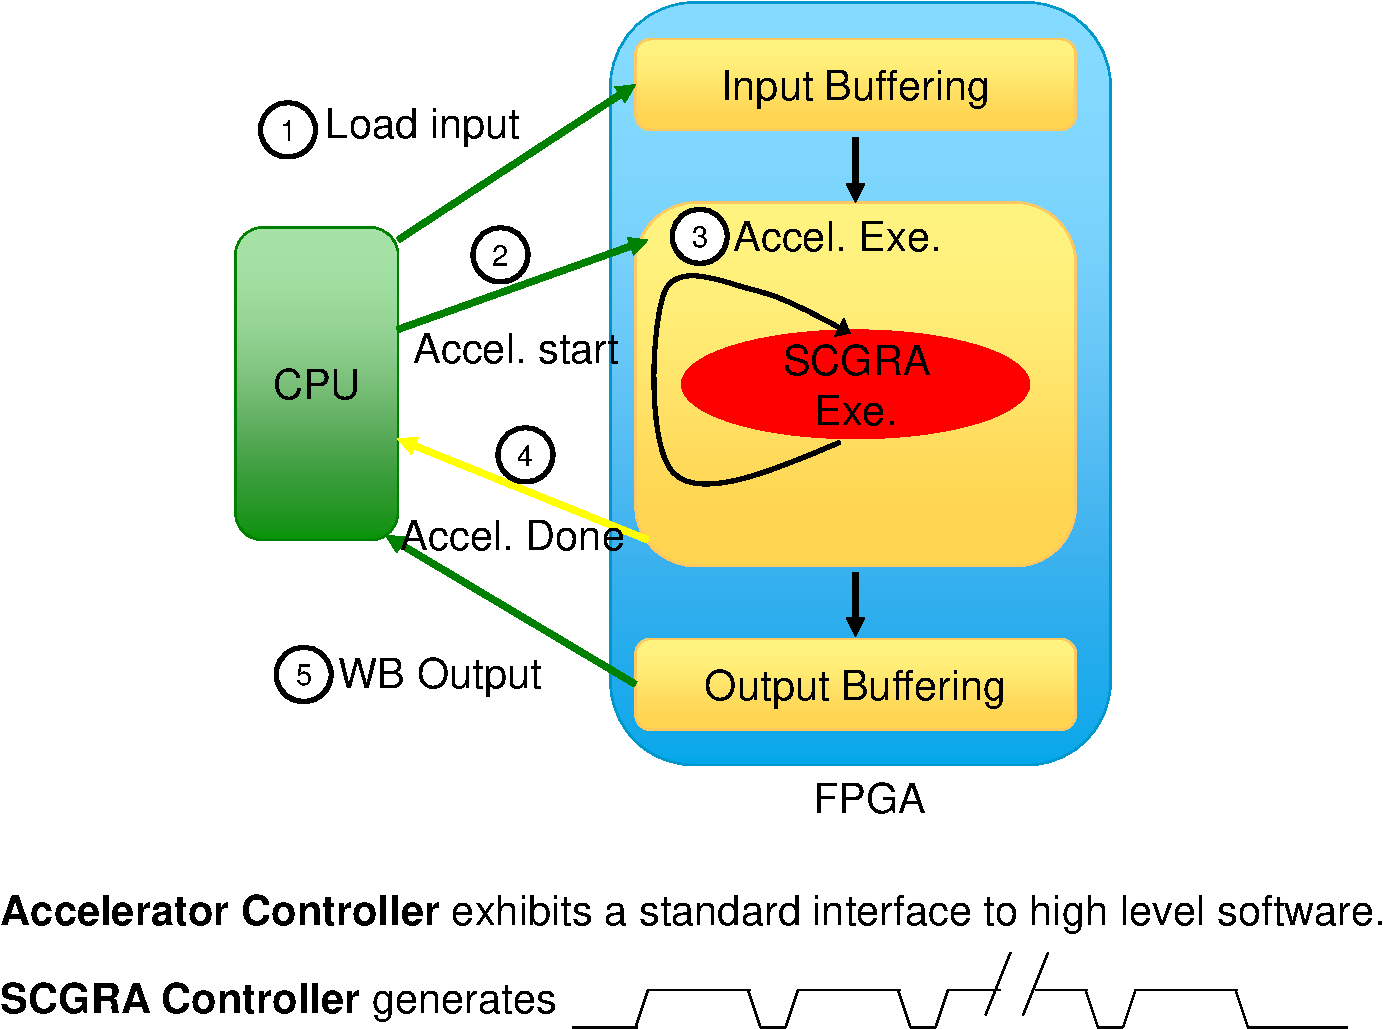
\includegraphics[width=.75\linewidth]{controller}
  \end{figure}
  \end{frame}

  \begin{frame}
  \frametitle{Loop Execution on the Accelerator}
  \begin{figure}
    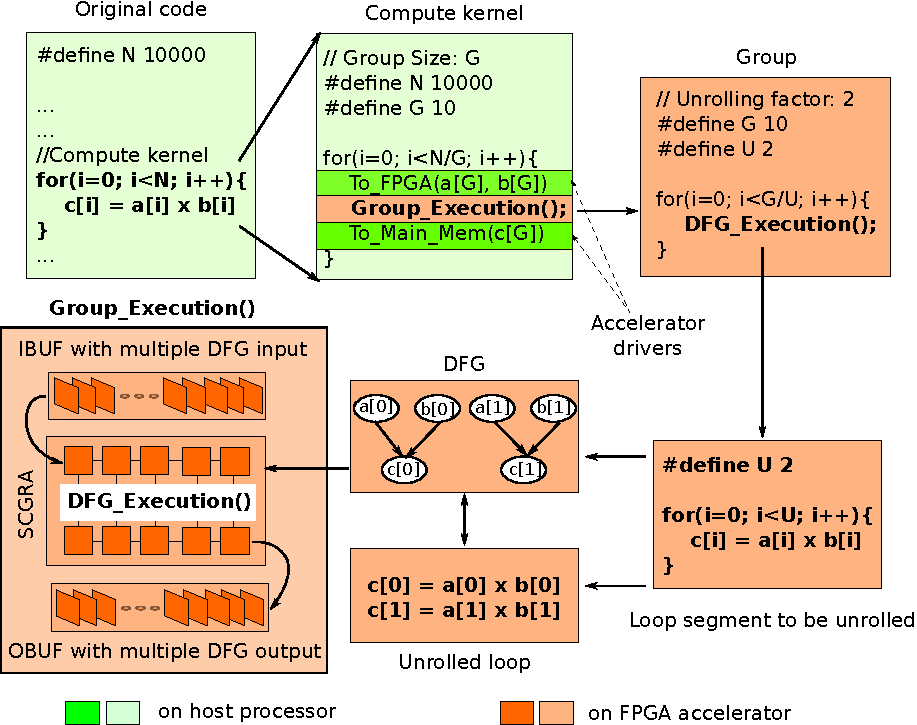
\includegraphics[width=.75\linewidth]{dfg-gen}
  \end{figure}
  \end{frame}

\section{Loop Accelerator Customization}
  \begin{frame}
  \frametitle{Outline}
  \begin{itemize}
  \setlength{\itemsep}{6pt}
  \item Background \& Motivation
  \item Related Work
  \item QuickDough Design Framework
  \item SCGRA Overlay Design \& Implementation
  \item \textbf{FPGA Loop Accelerator Customization}
  \item Experiments
  \begin{itemize}
    \setlength{\itemsep}{6pt}
    \item SCGRA Overlay Architecture
    \item Loop Accelerator Generation
    \item Loop Accelerator Customization
  \end{itemize}
  \item Conclusion
  \end{itemize}
  \end{frame}

  \begin{frame}
  \frametitle{Automatic Loop Accelerator Customization}
  \vspace{-1em}
  Why customization?
  \begin{itemize}
    \item difficult for high-level designers to decide the parameters
    \item critical to achieve good \textbf{performance \& energy efficiency}
    \item ...
  \end{itemize}

  \vspace{0.1em}
  What to customize?
  \begin{figure}
     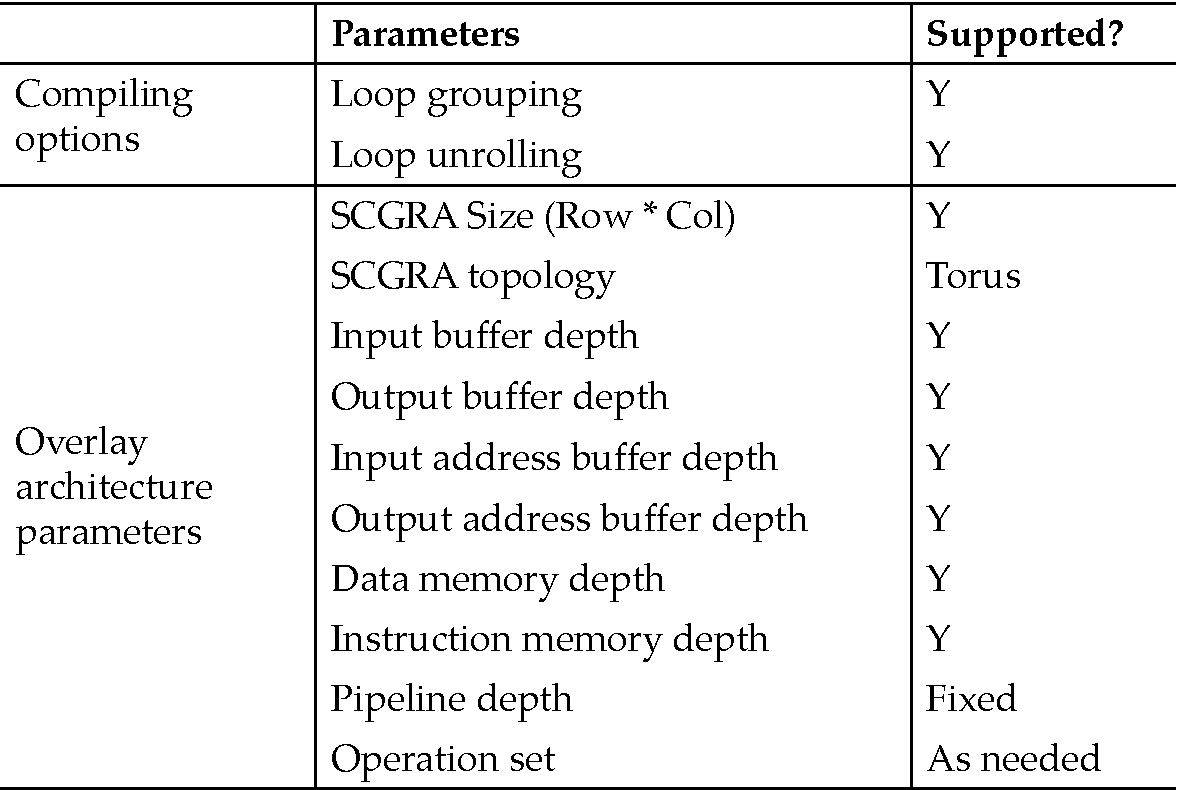
\includegraphics[width=.7\linewidth]{custom-para}
  \end{figure}
  \end{frame}

  \begin{frame}
  \frametitle{Loop Accelerator Modeling}
  \vspace{-0.7em}
  \begin{figure}
     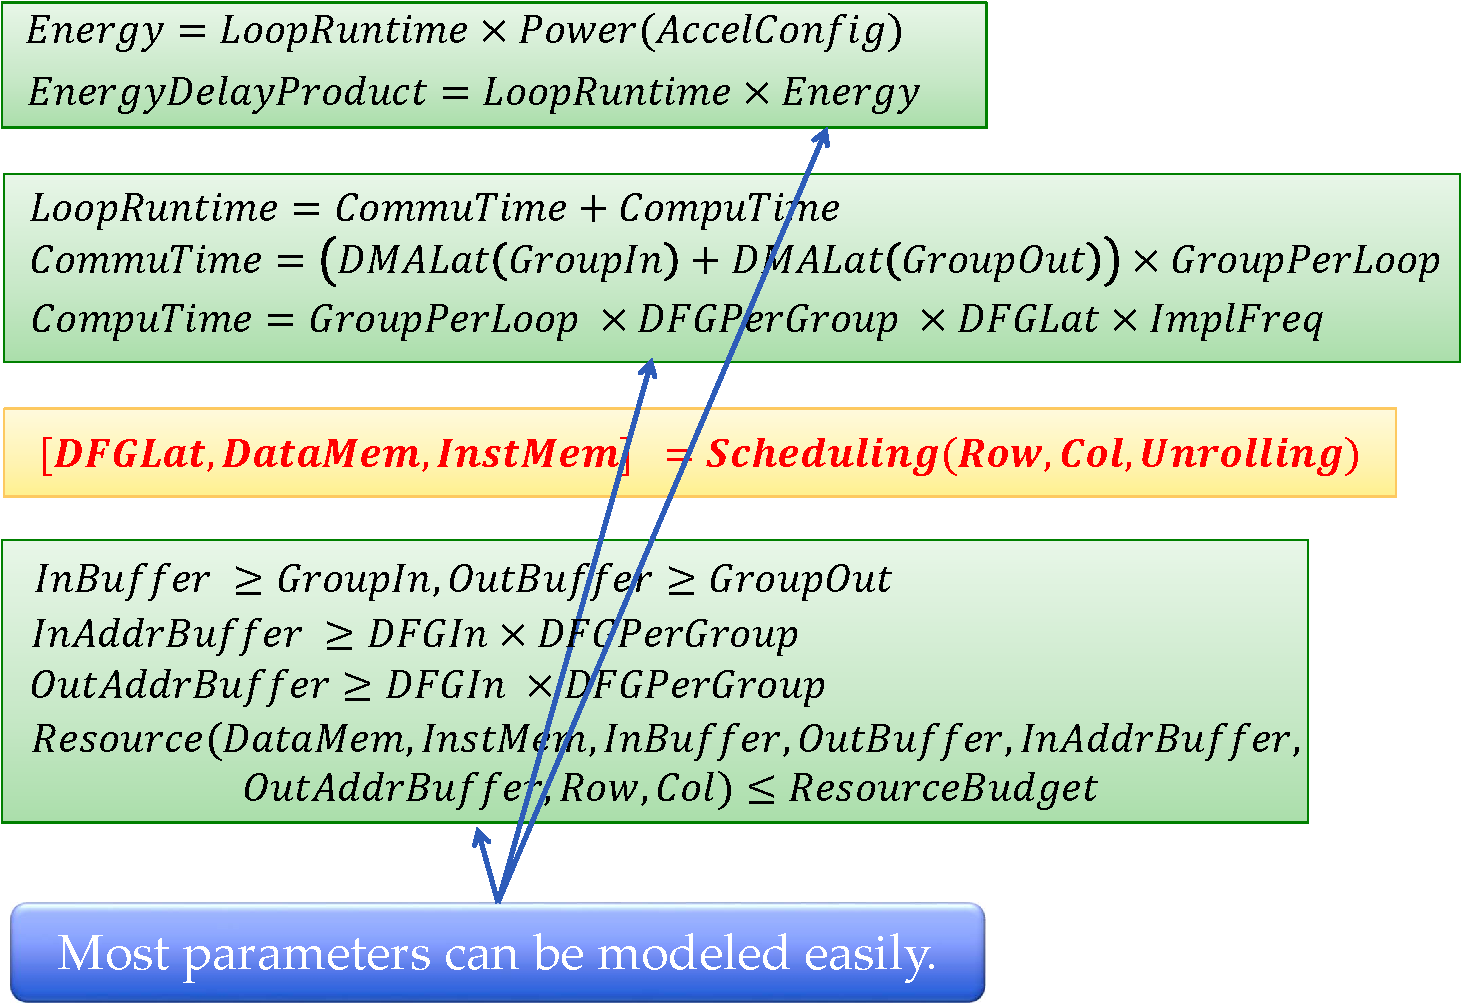
\includegraphics[width=.9\linewidth]{custom-model}
  \end{figure}
  \end{frame}

  \begin{frame}
  \frametitle{Two-step Customization Strategy}
  \vspace{-1em}
  \begin{figure}
     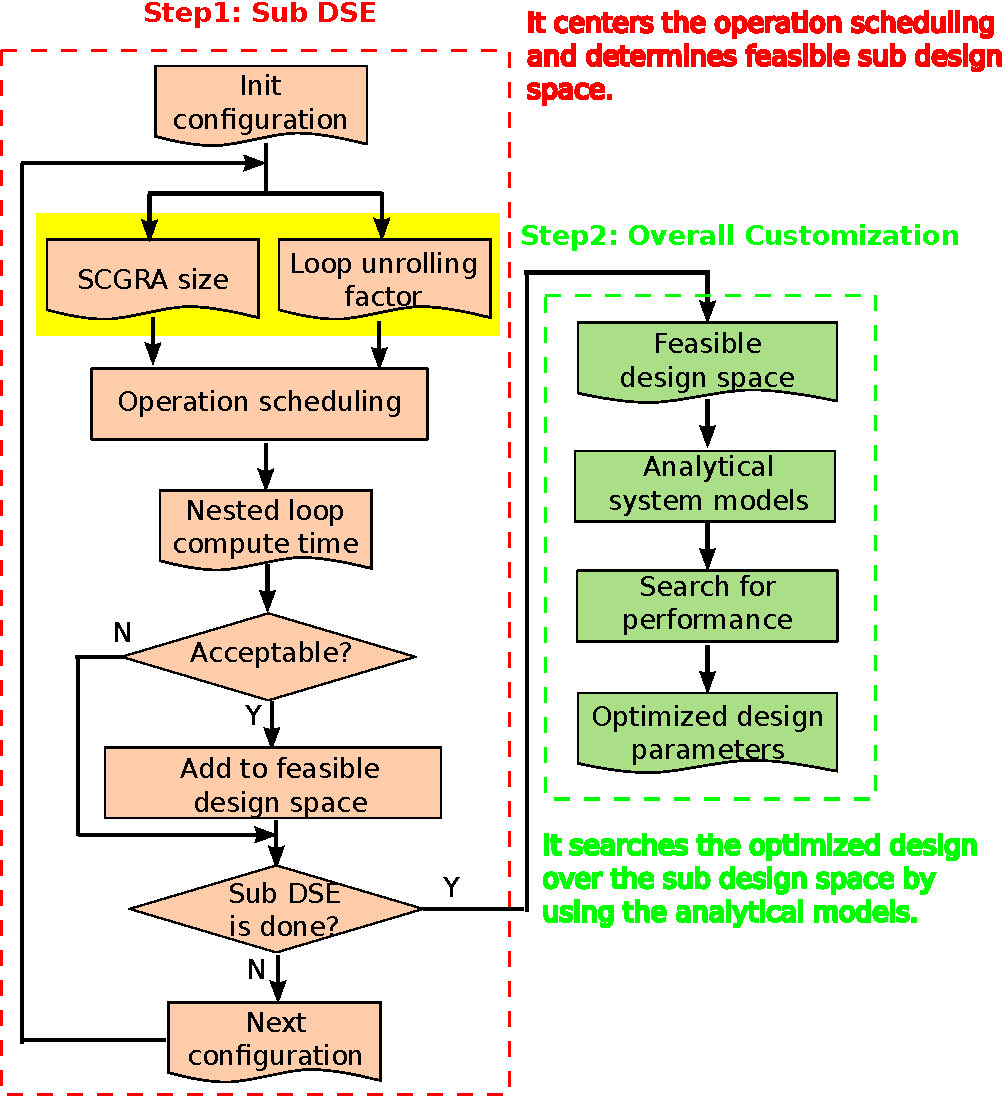
\includegraphics[width=.6\linewidth]{customization-framework}
  \end{figure}
  \end{frame}

  \begin{frame}
  \frametitle{Sub Design Space Exploration}
  \vspace{-0.7em}
  \begin{figure}
     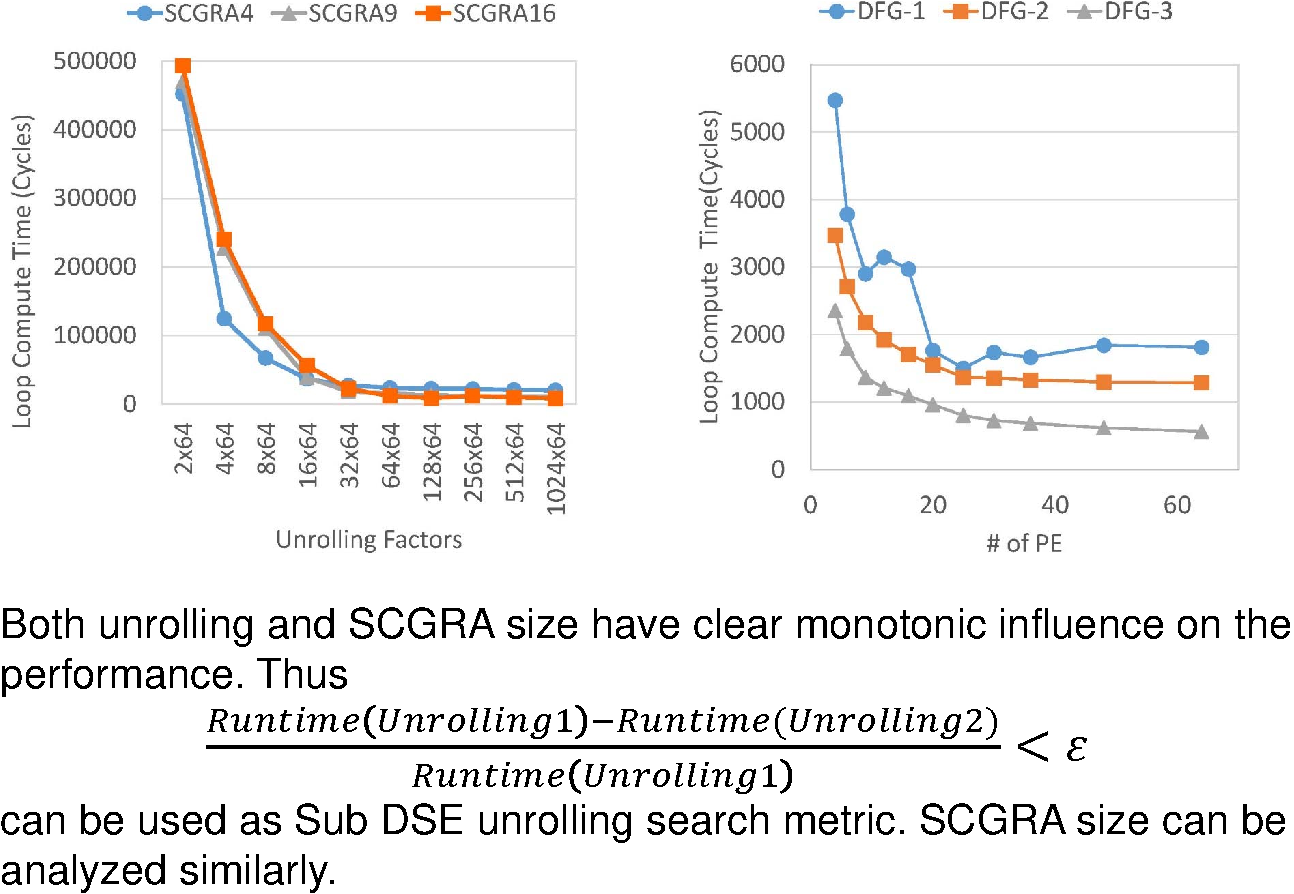
\includegraphics[width=.8\linewidth]{sub-dse}
  \end{figure}
  \end{frame}

\section{Experiments}
  \begin{frame}
  \frametitle{Outline}
  \begin{itemize}
  \setlength{\itemsep}{6pt}
  \item Background \& Motivation
  \item Related Work
  \item QuickDough Design Framework
  \item SCGRA Overlay Design \& Implementation
  \item FPGA Loop Accelerator Customization
  \item \textbf{Experiments}
  \begin{itemize}
    \setlength{\itemsep}{6pt}
    \item \textbf{SCGRA Overlay Architecture}
    \item Loop Accelerator Generation
    \item Loop Accelerator Customization
  \end{itemize}
  \item Conclusion
  \end{itemize}
  \end{frame}

  \begin{frame}
  \frametitle{Benchmark \& Experiment Setup}
  \vspace{-1em}
  \begin{figure}
    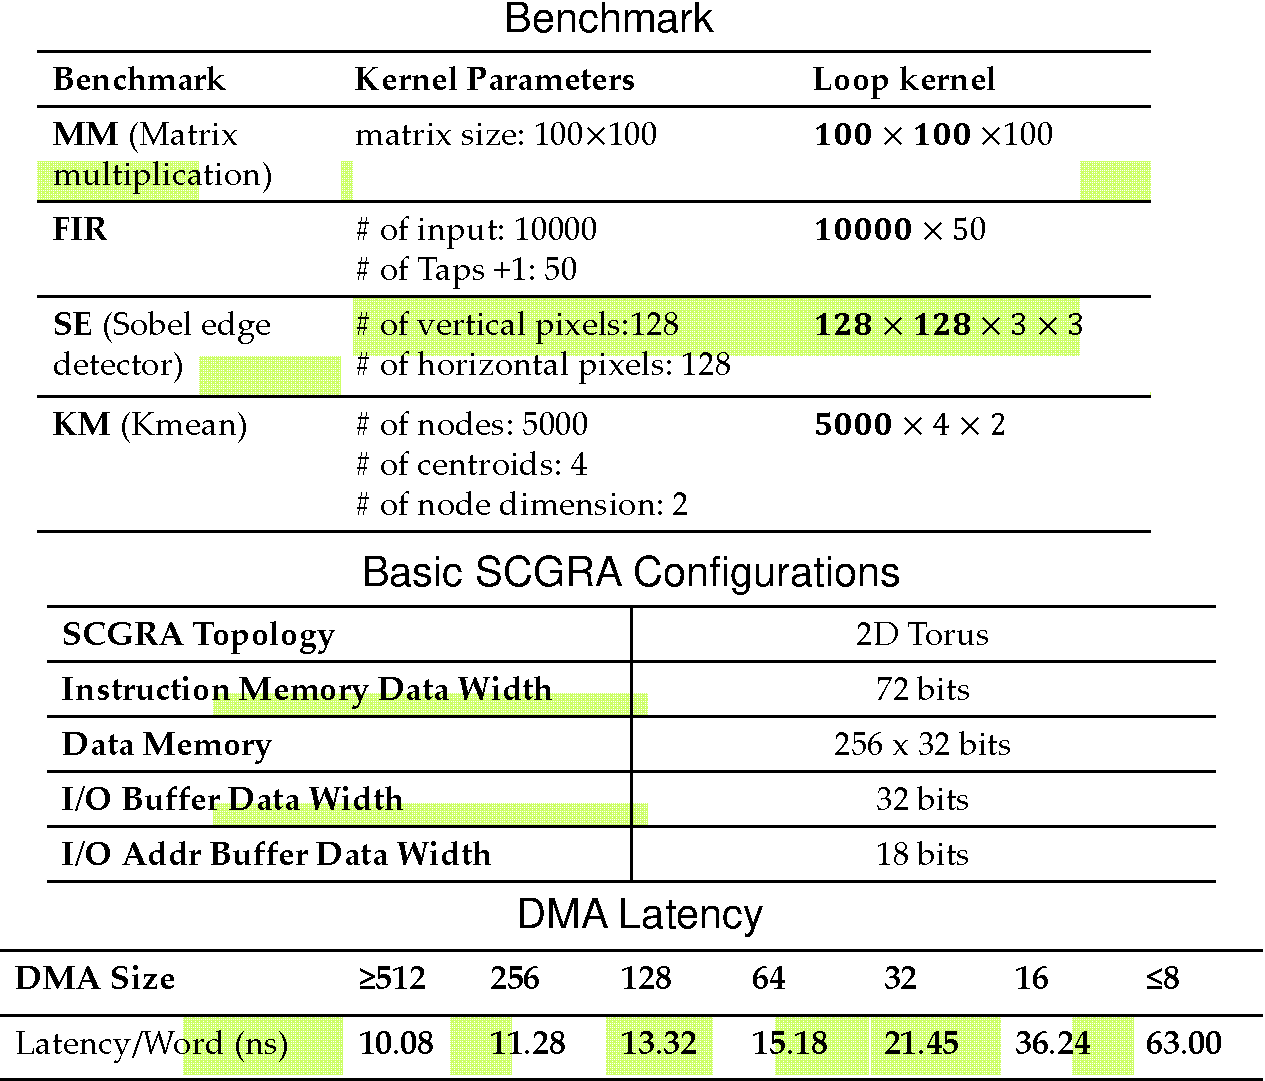
\includegraphics[width=.75\linewidth]{benchmark-setup}
  \end{figure}
  \end{frame}

  \begin{frame}
  \frametitle{SCGRA Overlay Pipelining Setup}
  \begin{table}[h]
  \footnotesize
  \caption{Pipeline Configurations}{
  \centering
    \begin{tabular}{c|c|c|c}
    \hline
    {Pipeline Options} & {\texttt{Input $\rightarrow$ Output}} & \tabincell{l}{\texttt{Input $\rightarrow$ Bypass} \\ \texttt{$\rightarrow$ Output}} & {\texttt{Input $\rightarrow$ Write Back}} \\ \hline
    {100MHz} & {2 cycles} & {1 cycle} & {4\~{}6 cycles} \\ \hline
    {150MHz} & {2 cycles} & {1 cycle} & {5\~{}8 cycles} \\ \hline
    {200MHz} & {4 cycles} & {2 cycles} & {7\~{}11 cycles} \\ \hline
    {250MHz} & {7 cycles} & {3 cycles} & {11\~{}17 cycles} \\ \hline
    \end{tabular}
  }
  \end{table}

  \begin{table}
  \footnotesize
  \centering
  \caption{DFG Information (\# of Input/ \# of Output/ \# of Operations) 
  \label{tab:dfg-info}}{
  \centering
    \begin{tabular}{l|l|l|l|l}
    \hline
    Configurations & MM & FIR & SE & KM \\ \hline
    C1 & 200/100/1000 & 70/20/860 & 31/8/1080 & 49/12/920 \\ \hline
    C2 & 600/5/750 & 120/20/1000 & 31/8/1080 & 59/12/1144 \\ \hline
    C3 & 400/1/301 & 120/20/1000 & 27/4/540 & 59/12/1144 \\ \hline
    \end{tabular}
  }
  \end{table}
  \end{frame}

  \begin{frame}
  \frametitle{Pipelining Influence on SCGRA 2$\times$2 Performance}
  \begin{figure}
    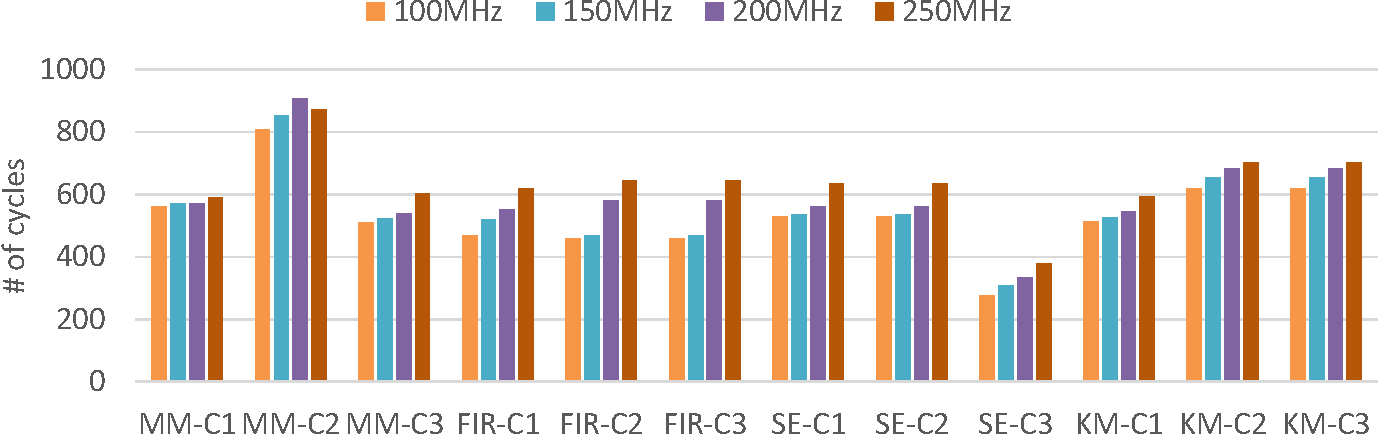
\includegraphics[width=0.8\linewidth]{pipeline-cgra2x2-sim-perf}
  \end{figure}
  \begin{figure}
    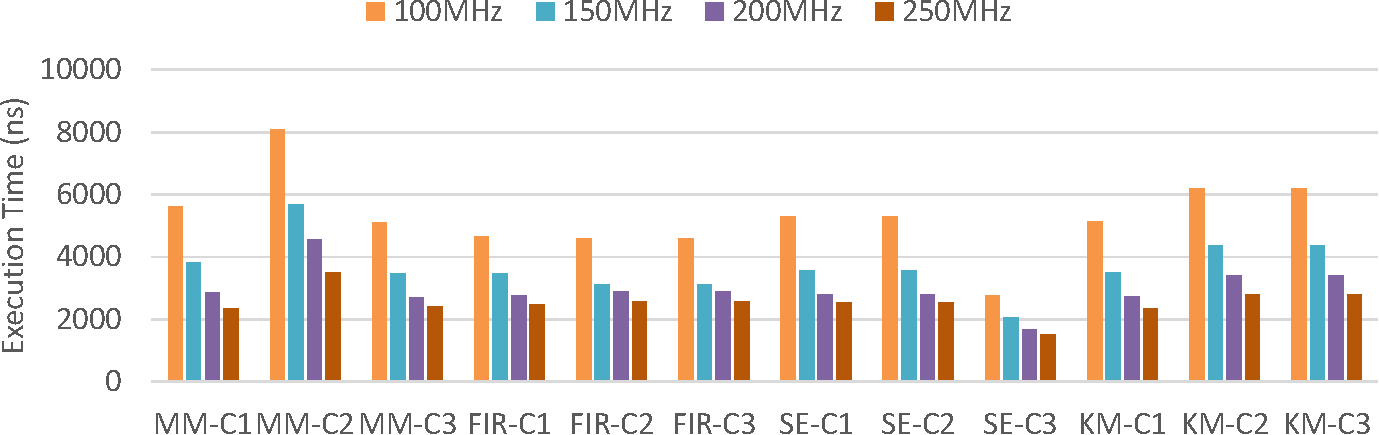
\includegraphics[width=0.8\linewidth]{pipeline-cgra2x2-real-perf}
  \end{figure}
  \end{frame}

  \begin{frame}
  \frametitle{Pipelining Influence on SCGRA 5$\times$5 Performance}
  \vspace{-1em}
  \begin{figure}
    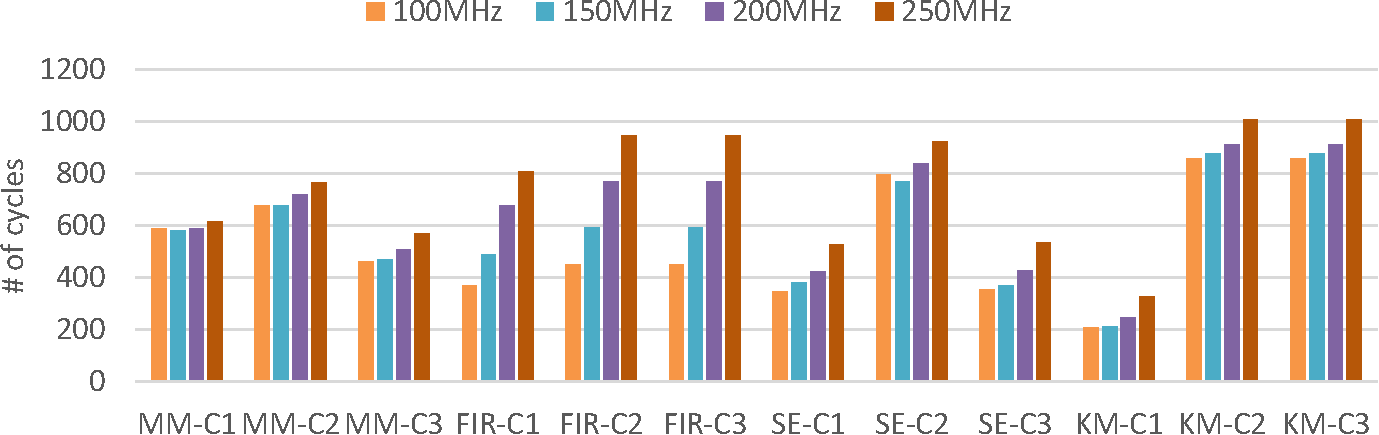
\includegraphics[width=0.8\linewidth]{pipeline-cgra5x5-sim-perf}
  \end{figure}
  \begin{figure}
    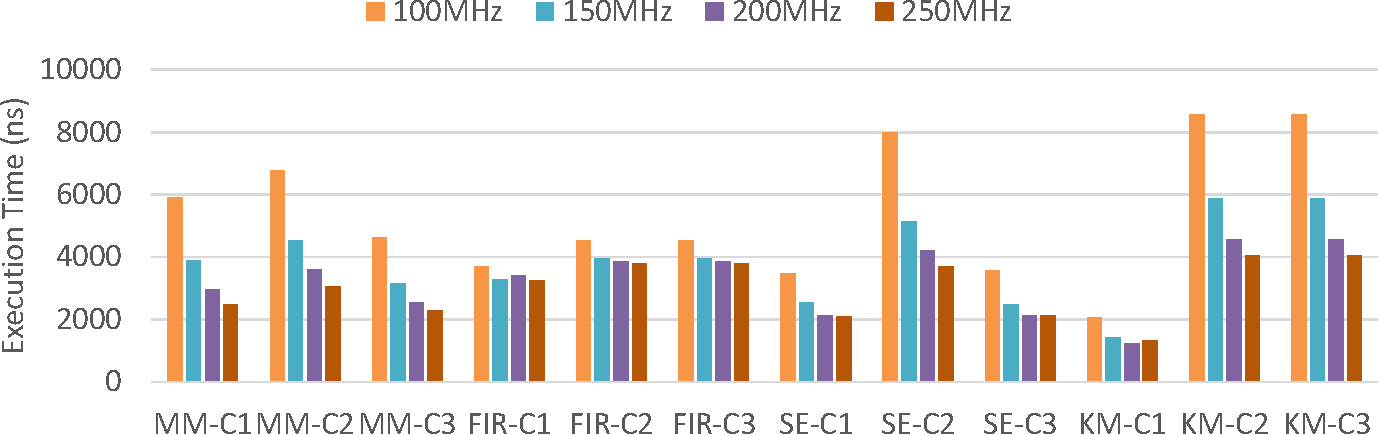
\includegraphics[width=0.8\linewidth]{pipeline-cgra5x5-real-perf}
  \end{figure}

  \centering{
  \fbox{
    \parbox{0.85\textwidth}{
      \textbf{\color{red}{Deep pipelining usually incur larger amount of computing cycles, 
\\ but it is typically beneficial to the overall performance.}}
    }
  }
  }
  \end{frame}

  \begin{frame}
  \frametitle{Outline}
  \begin{itemize}
  \setlength{\itemsep}{6pt}
  \item Background \& Motivation
  \item Related Work
  \item QuickDough Design Framework
  \item SCGRA Overlay Design \& Implementation
  \item FPGA Loop Accelerator Customization
  \item \textbf{Experiments}
  \begin{itemize}
    \setlength{\itemsep}{6pt}
    \item SCGRA Overlay Architecture
    \item \textbf{Loop Accelerator Generation}
    \item Loop Accelerator Customization
  \end{itemize}
  \item Conclusion
  \end{itemize}
  \end{frame}

  \begin{frame}
  \frametitle{Experiment Setup}
  \vspace{-1em}
  \begin{figure}
    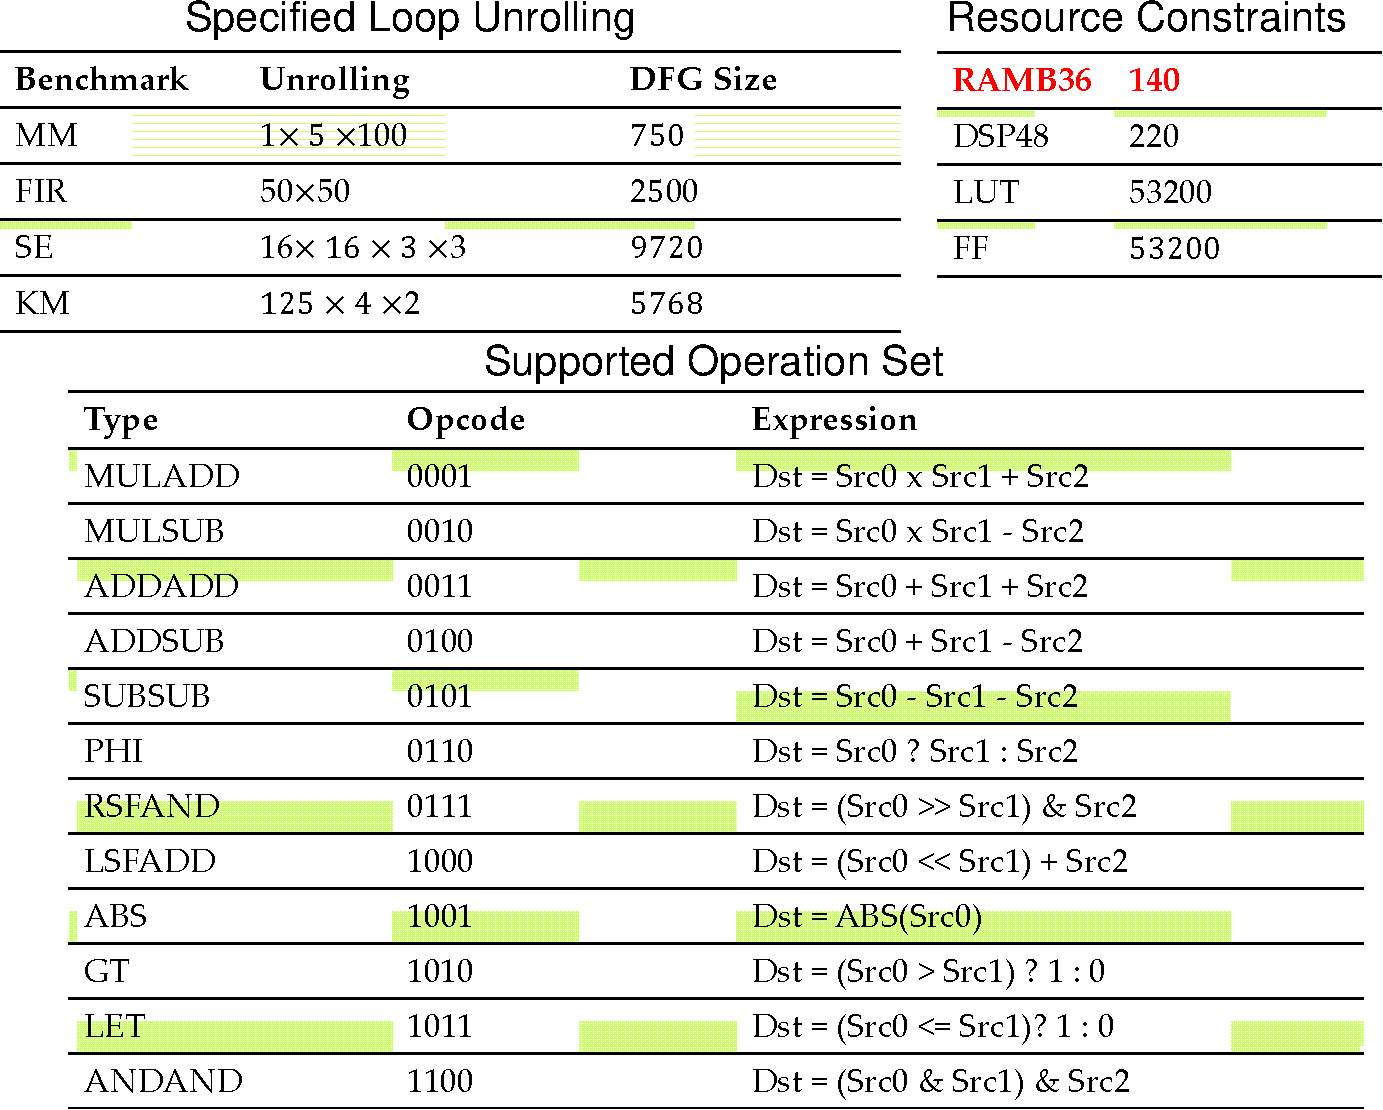
\includegraphics[width=0.8\linewidth]{compile-setup}
  \end{figure}
  \end{frame}

  \begin{frame}
  \frametitle{Resulting Accelerator Configurations}
  \begin{figure}
    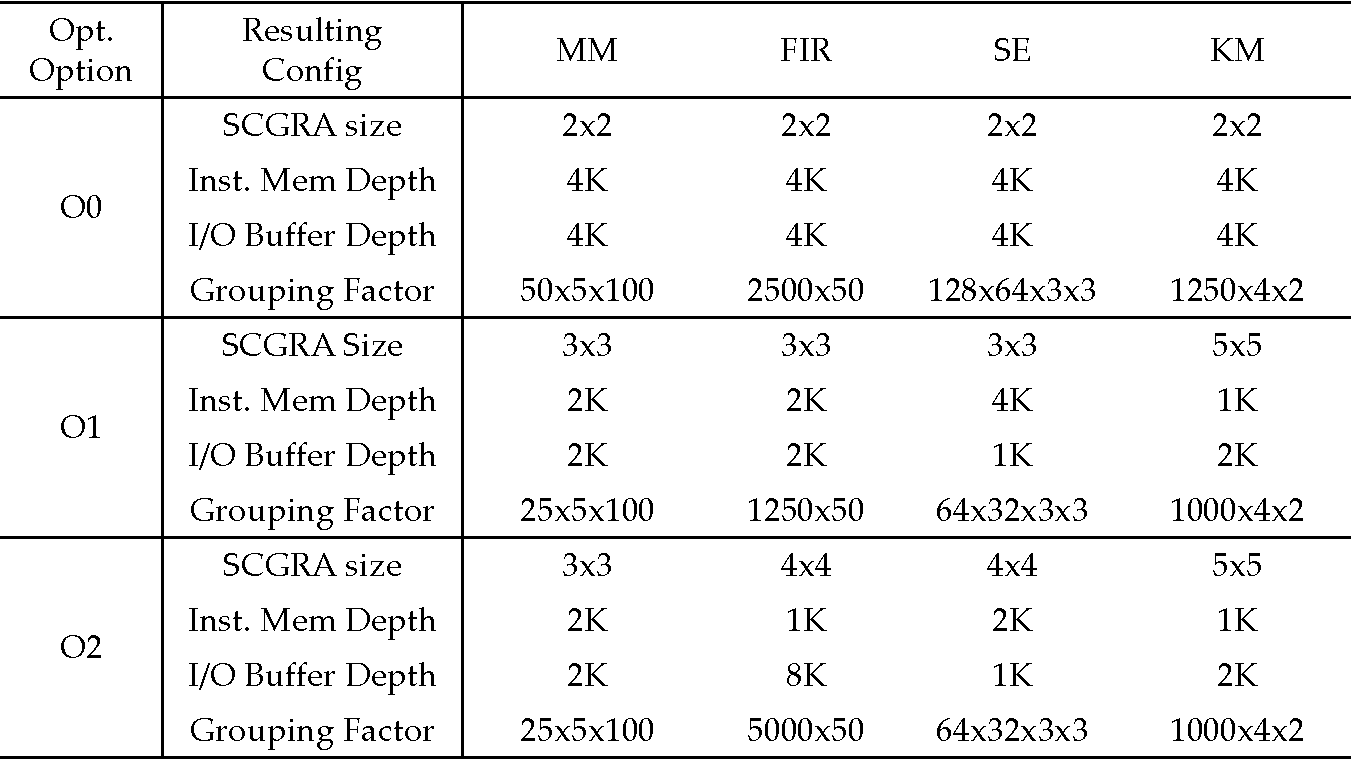
\includegraphics[width=0.9\linewidth]{accel-config}
  \end{figure}
  \end{frame}

  \begin{frame}
  \frametitle{Performance of the Resulting Accelerators}
  \vspace{-1em}
  \begin{figure}
  \centering
  \subfigure[MM]{
  \label{fig:mm-real-perf}
  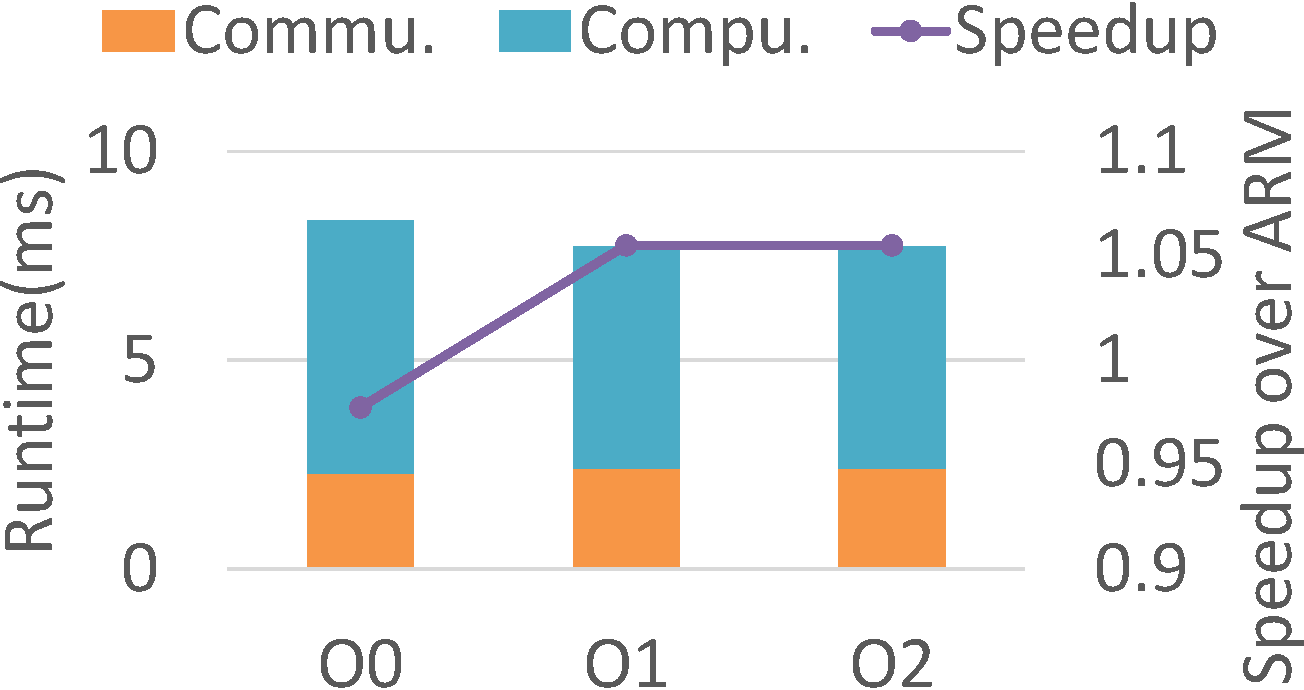
\includegraphics[width=0.44\linewidth]{mm-perf}}
  \qquad
  \subfigure[FIR]{
  \label{fig:fir-real-perf}
  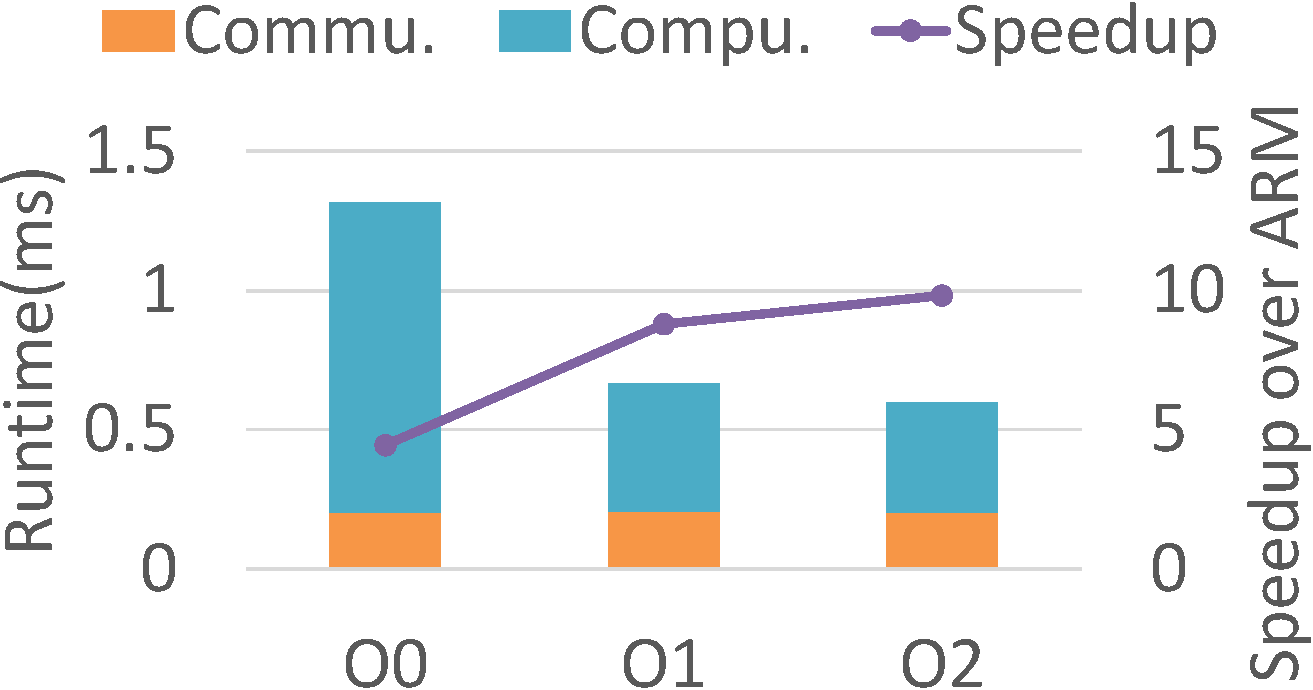
\includegraphics[width=0.44\linewidth]{fir-perf}}
  \qquad
  \subfigure[SE]{
  \label{fig:sobel-real-perf}
  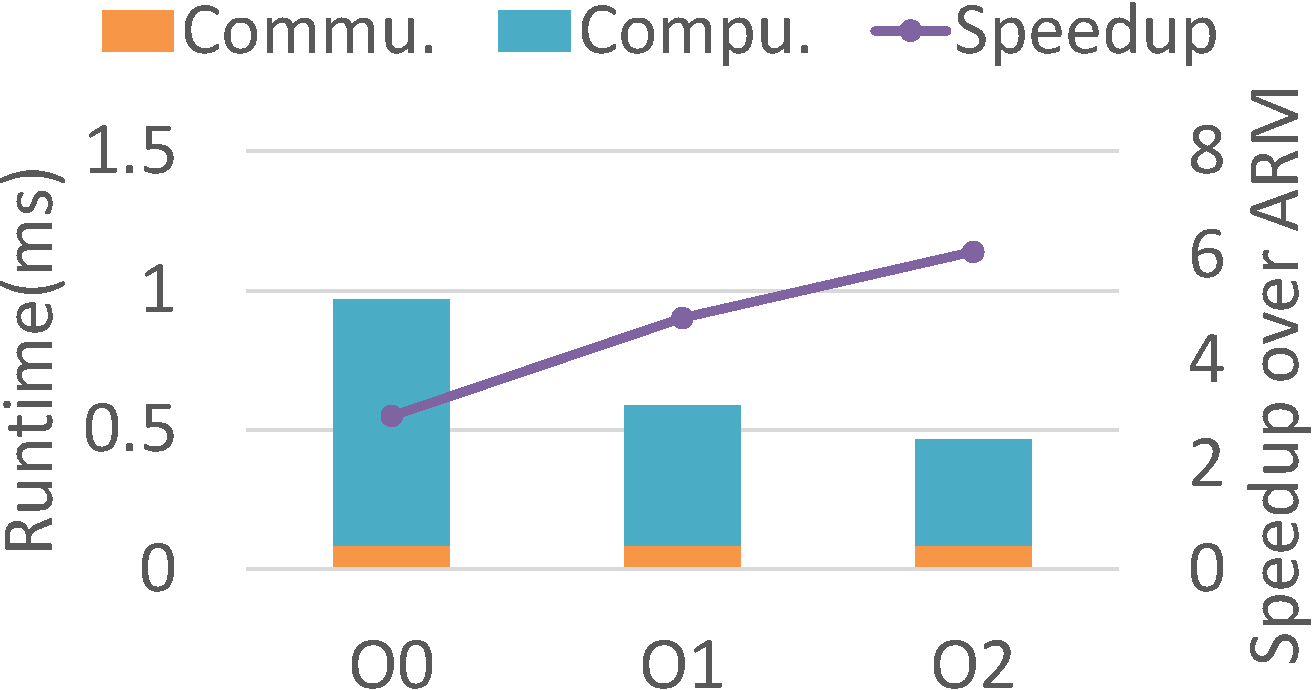
\includegraphics[width=0.44\linewidth]{se-perf}}
  \qquad
  \subfigure[KM]{
  \label{fig:kmean-real-perf}
  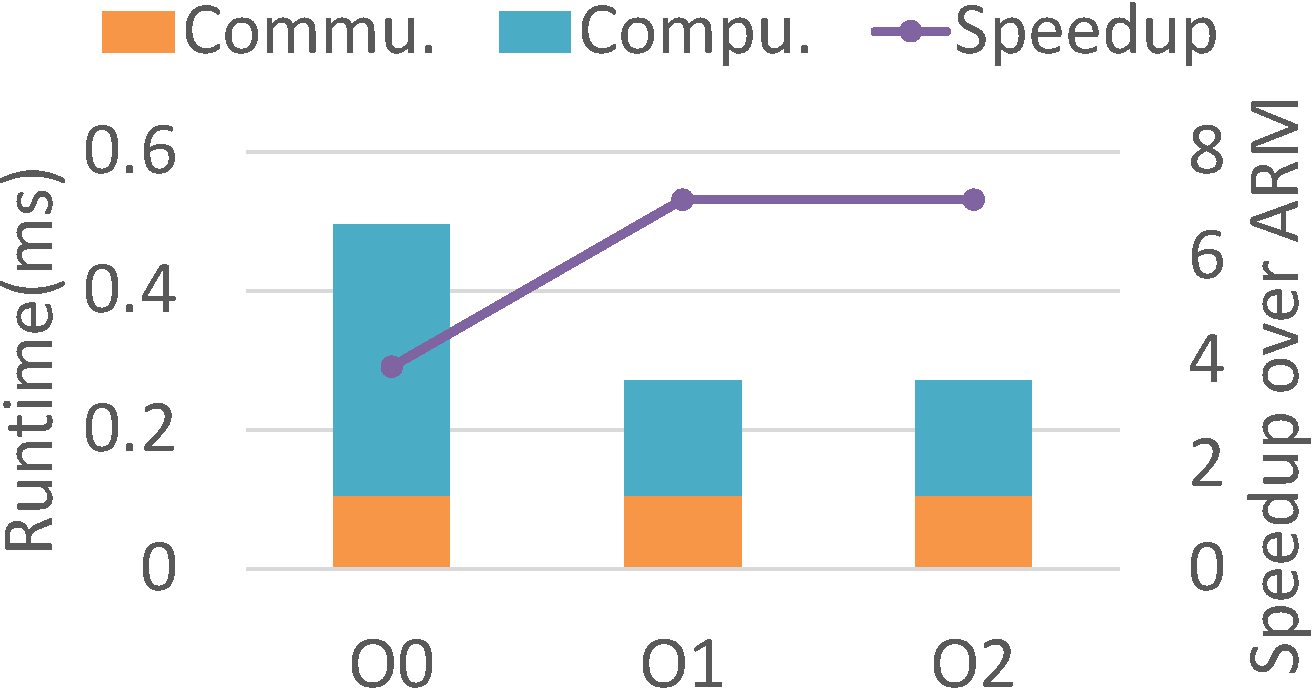
\includegraphics[width=0.44\linewidth]{km-perf}}
  \vspace{-0.8em}
  \caption{Benchmark performance speedup over software executed on ARM processor and execution time 
      decomposition of loop accelerators generated using QuickDough.}
  \label{fig:real-perf}
  \end{figure}  
  \end{frame}

  \begin{frame}
  \frametitle{Time Consumption of the Loop Accelerator Generation}
  \vspace{-0.8em}
  With the pre-built library, each design iteration in QuickDough involves 3 steps:
  \begin{itemize}
    \item DFG generation
    \item Accelerator selection and DFG scheduling
    \item Bitstream generation
  \end{itemize}
  \begin{figure}
    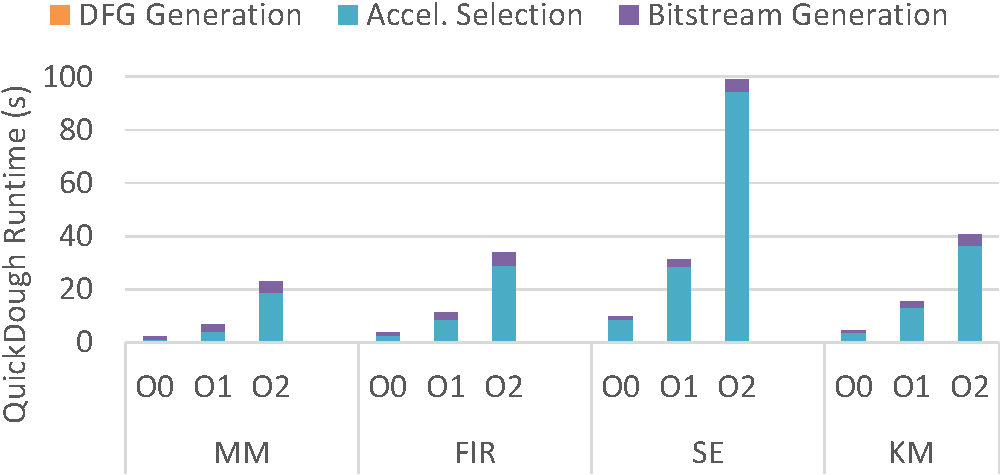
\includegraphics[width=0.8\linewidth]{quickdough-runtime}
  \end{figure}
  \end{frame}

  \begin{frame}
  \frametitle{Accelerator Library Pre-building Time}
  \begin{figure}
  \centering
  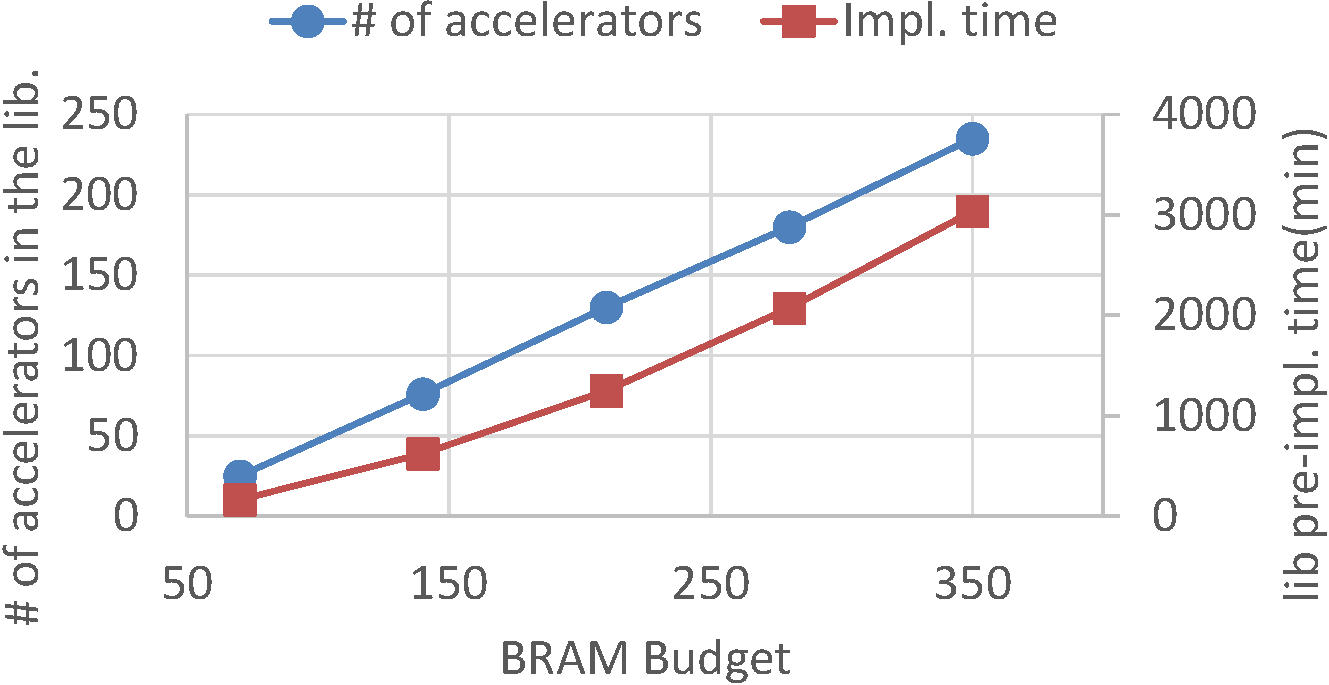
\includegraphics[width=0.6\linewidth]{lib-impl-time}
  \caption{Accelerator library size and implementation time given different BRAM budgets.}
  \label{fig:lib-impl-time}
  \begin{itemize}
  \item \color{red}{With simple empirical constraints, the accelerator library pre-building time will not increase dramatically with the BRAM budgets. }
  \item \color{red}{The implementations are completely independent and can be done on a distributed computing system with much shorter time.}
  \end{itemize}
  \end{figure}
  \end{frame}


  \begin{frame}
  \frametitle{Outline}
  \begin{itemize}
  \setlength{\itemsep}{6pt}
  \item Background \& Motivation
  \item Related Work
  \item QuickDough Design Framework
  \item SCGRA Overlay Design \& Implementation
  \item FPGA Loop Accelerator Customization
  \item \textbf{Experiments}
  \begin{itemize}
    \setlength{\itemsep}{6pt}
    \item SCGRA Overlay Architecture
    \item Loop Accelerator Generation
    \item \textbf{Loop Accelerator Customization}
  \end{itemize}
  \item Conclusion
  \end{itemize}
  \end{frame}

  \begin{frame}
  \frametitle{Experiment Setup}
  Basic setup:
  \begin{itemize}
    \item The resources on Zedboard are taken as the constraints.
    \item $\epsilon = 0.05$ 
    \item FPGA accelerator performance are calculated using the models. 
    \item ARM processor performance are obtained from Zedboard.
    \item Power consumption is extracted from XPower. 
    \item Exhaustive search (ES) and the two-step (TS) customization methods are used.
  \end{itemize}
  \vspace{1em}
  Assumptions used for the customization:
  \begin{itemize}
  \item All the overlay based accelerators run at 250 MHz on Zedboard.
  \end{itemize}
  \end{frame}

  \begin{frame}
  \frametitle{Resulting Accelerator Configurations}
  \vspace{-1em}
  \begin{table}[htb]
    \footnotesize
    \centering
    \caption{Accelerator configurations (Note that the configurations include loop unrolling factor, grouping factor, SCGRA array size, instruction memory depth and IO buffer depth) \label{tab:acc-config}}{
        \begin{tabular}{l|l|l}
            \hline
            \multirow{3}{*}{MM}  & Base & ($1 \times 2 \times 100$, $4 \times 2 \times 100$, $5
        \times 5$, 1k, 2k)\\ \cline{2-3}
                                 & TS & ($1 \times 5 \times 100$, $50 \times 5 \times 100$, $4
        \times 4$, 1k, 8k)\\ \cline{2-3}
                                 & ES & ($1 \times 5 \times 100$, $25 \times 5 \times 100$, $5
        \times 4$, 1k, 8k)\\ \hline
            \multirow{3}{*}{FIR}  & Base & ($ 10 \times 50$, $100 \times 50$, $3
        \times 3$, 1k, 2k)\\ \cline{2-3}
                                 & TS & ($50 \times 50$, $2000 \times 50 $, $4
        \times 4$, 1k, 4k)\\ \cline{2-3}
                                 & ES & ($100 \times 50$, $5000 \times 50$, $5
        \times 4$, 1k, 8k)\\ \hline
            \multirow{3}{*}{SE}  & Base & ($4 \times 4 \times 3 \times 3$, $128 \times 128 \times 3
        \times 3$, $3 \times 2$, 1k, 8k)\\ \cline{2-3}
                                 & TS & ($16 \times 16 \times 3 \times 3$, $128 \times 128 \times 3
        \times 3$, $4 \times 4$, 1k, 4k)\\ \cline{2-3}
                                 & ES & ($16 \times 16 \times 3 \times 3$, $128 \times 128 \times 3
        \times 3$, $5 \times 4$, 1.5k, 4k)\\ \hline
            \multirow{3}{*}{KM}  & Base & ($25 \times 4 \times 2$, $2500 \times 4 \times 2$, $4
        \times 3$, 1k, 8k)\\ \cline{2-3}
                                 & TS & ($125 \times 4 \times 2$, $625 \times 4 \times 2$, $5
        \times 5$, 1k, 2k)\\ \cline{2-3}
                                 & ES & ($125 \times 4 \times 2$, $625 \times 4 \times 2$, $5
        \times 5$, 1k, 2k)\\ \hline

        \end{tabular}
    }
  \end{table}
  \end{frame}

  \begin{frame}
  \frametitle{Exhaustive search (ES) vs. two-step customization (TS)}
  \vspace{1em}
  \begin{figure}[htb]
    \centering
    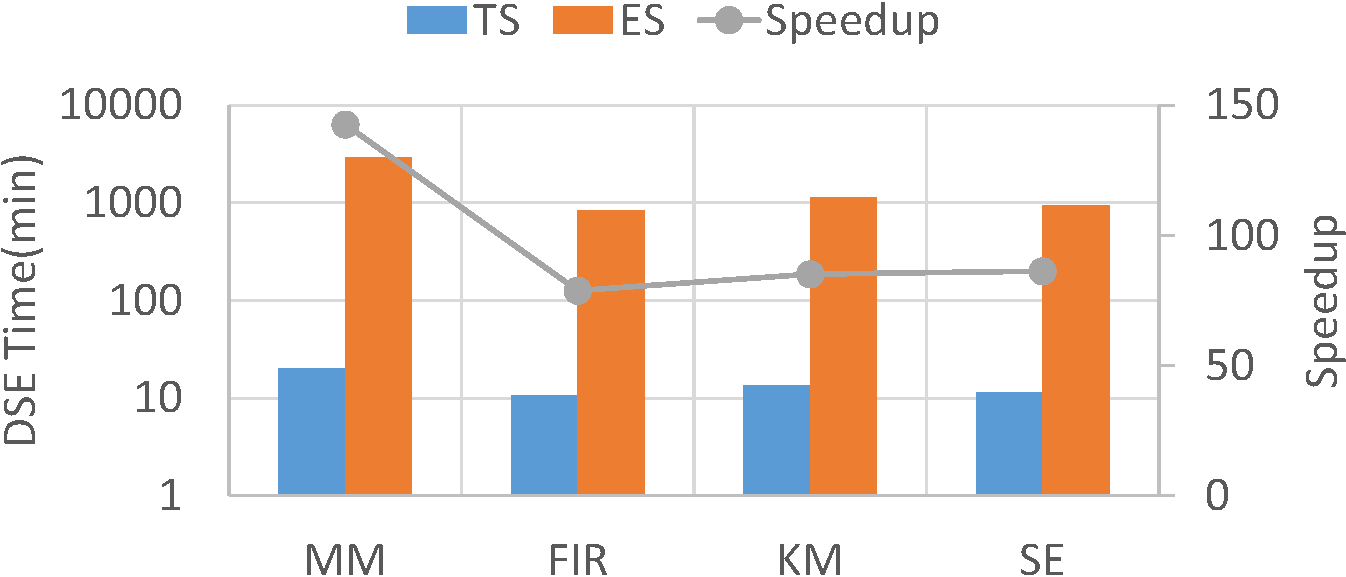
\includegraphics[width=0.7\textwidth]{DSE-Time}
    \caption{Customization Time Using Both TS and ES}
    \label{fig:DSE-Time}
  \end{figure}
  \end{frame}

  \begin{frame}
  \frametitle{Exhaustive search (ES) vs. two-step customization (TS)}
  \vspace{-1em}
  \begin{figure}[htb]
  \centering
	\subfigure[MM]{%
		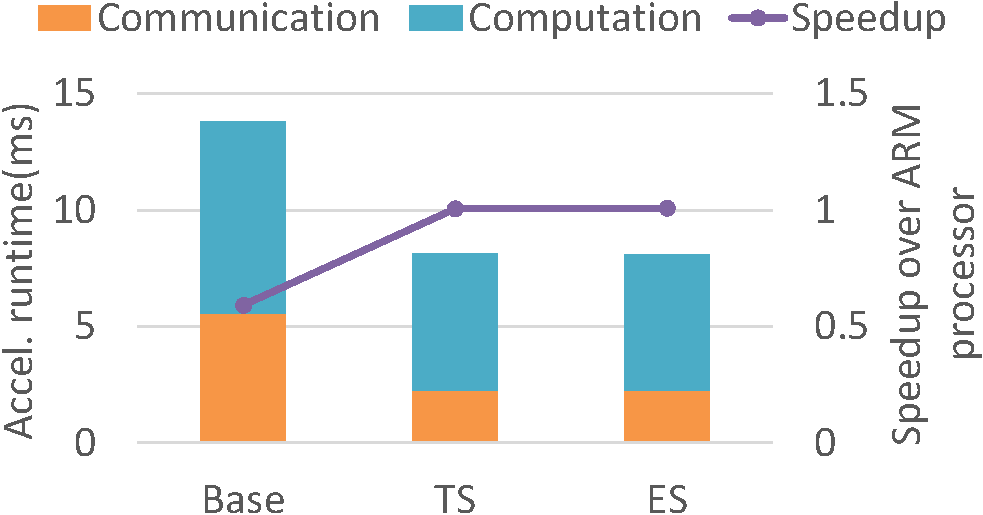
\includegraphics[width=0.45\textwidth]{mm-cp}
	}
	\subfigure[FIR]{%
		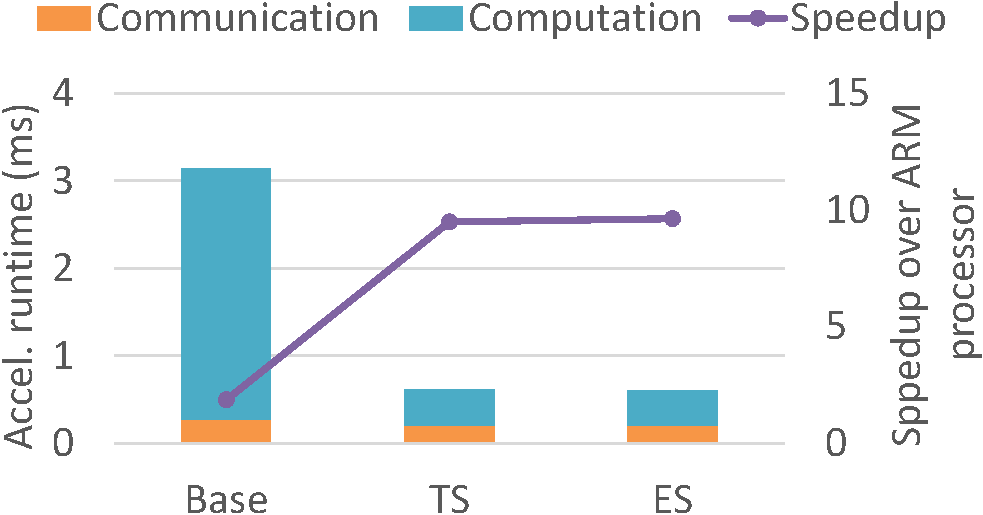
\includegraphics[width=0.45\textwidth]{fir-cp}
	}
    \hfill
	\subfigure[SE]{%
		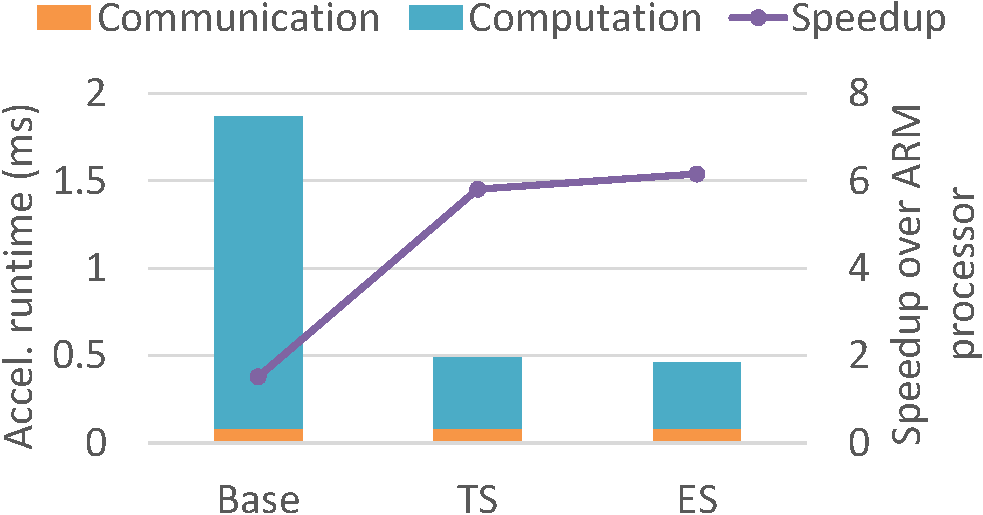
\includegraphics[width=0.45\textwidth]{se-cp}
	}
	\subfigure[KM]{%
		\includegraphics[width=0.45\textwidth]{km-cp}
	}
    \vspace{-0.6em}
    \caption{Customized FPGA Loop Accelerator Performance Comparison}
  \label{fig:DSE}
  \end{figure}

  \end{frame}

  \begin{frame}
  \frametitle{Outline}
  \begin{itemize}
  \setlength{\itemsep}{6pt}
  \item Background \& Motivation
  \item Related Work
  \item QuickDough Design Framework
  \item SCGRA Overlay Design \& Implementation
  \item FPGA Loop Accelerator Customization
  \item Experiments
  \begin{itemize}
    \setlength{\itemsep}{6pt}
    \item SCGRA Overlay Architecture
    \item Loop Accelerator Generation
    \item Loop Accelerator Customization
  \end{itemize}
  \item \textbf{Conclusion}
  \end{itemize}
  \end{frame}
  
  \begin{frame}
  \frametitle{Conclusion}
  \setlength{\itemsep}{6pt}
  \begin{itemize}
  \item Presented the QuickDough compilation framework for high productivity FPGA loop accelerator design on a hybrid CPU-FPGA computing system.
  \item Implemented a highly pipelined, flexible and scalable SCGRA overlay on top of FPGAs which contributes to the good performance of the resulting accelerators as well as the capability of application specific customization of QuickDough.  
  \item Taking advantage of the regularity of the SCGRA overlay, an automatic customization framework was developed to customize the design parameters of the resulting accelerators.
  \end{itemize}
  \end{frame}

\section{Backup Slides}
  \subsection{SCGRA Overlay Scalability}
  \begin{frame}
  \frametitle{SCGRA Overlay Scalability (1)}
  \vspace{-1em}
  \begin{figure}
  \centering
  \subfigure[]{
  \label{fig:mm-sim-perf1}
  \includegraphics[width=0.65\linewidth]{mm-sim-perf1}}
  \hfill
  \subfigure[]{
  \label{fig:mm-sim-perf2}
  \includegraphics[width=0.65\linewidth]{mm-sim-perf2}}
  \vspace{-0.8em}
  \caption{\# of cycles of MM Execution on Both HLS Based Design and SCGRA Overlay}
  \label{fig:mm-sim-perf}
  \end{figure}
  \end{frame}

  \begin{frame}
  \frametitle{SCGRA Overlay Scalability(2)}
  \vspace{-1em}
  \begin{table}[tb]
    \scriptsize
    \centering
    \vspace{-0.5em}
    \caption{SCGRA Based FPGA Accelerator Configuration \label{tab:many-config}}{
        \begin{tabular}{c|c|c|c|c}
            \hline
            SCGRA Size & \tabincell{c}{Inst. Rom} & 
            \tabincell{c}{Data Mem} & \tabincell{c}{IBuf /OBuf} & 
            \tabincell{c}{Addr Buf} \\ \hline

            \tabincell{l}{2x2, 3x3, ..., 10x10} & \tabincell{l}{1k, 4k, ..., 8k}
            & 256x32 & 2kx32, 4kx32, ..., 8kx32 & 4kx16, 8kx16, ..., 16kx16 \\ \hline
        \end{tabular}
    }
  \end{table}

  \begin{figure}[tb]
  \center{\includegraphics[width=0.6\linewidth]{impl-scale}}
  \caption{fmax of SCGRA Overlay with Various Configurations}
  \label{fig:impl-scale}
  \end{figure}
  \end{frame}

  \subsection{Pipelining Influence on Power and Energy Efficiency}
  \begin{frame}
  \frametitle{Pipelining Influence on HW Resource Consumption}
  \begin{figure}
    \center{\includegraphics[width=0.8\linewidth]{pipeline-resource}}
  \end{figure}

  \begin{figure}
    \center{\includegraphics[width=0.5\linewidth]{pipeline-power}}
  \end{figure}
  \end{frame}

  \begin{frame}
  \frametitle{Pipelining Influence on Energy Efficiency}
  \vspace{-1em}
  \begin{figure}[htb]
  \centering
  \subfigure[SCGRA$2 \times 2$]{
    \includegraphics[width=0.75\linewidth]{pipeline-scgra2x2-edp}
  \label{fig:pipeline-scgra2x2-edp}
  }
  \hfill
  \subfigure[SCGRA $5 \times 5$]{
  \includegraphics[width=0.75\linewidth]{pipeline-scgra5x5-edp}
  \label{fig:pipeline-scgra5x5-edp}
  }
  \vspace{-0.6em}
  \caption{Energy Delay Product of SCGRA Overlays with Different Pipelining}
  \label{fig:pipeline-edp}
  \end{figure}
  \end{frame}

  \subsection{Accelerators Generated Using QuickDough}
  \begin{frame}
  \frametitle{Implementation of the Resulting Accelerators}
  \vspace{-1em}
  \begin{figure}[htb]
  \center{\includegraphics[width=0.5\linewidth]{impl-freq}}
  \vspace{-0.6em}
  \caption{fmax of the Accelerators in the Library}
  \label{fig:impl-freq}
  \end{figure}
  \vspace{-0.5em}
  \begin{figure}[htb]
  \vspace{1em}
  \center{\includegraphics[width=0.7\linewidth]{hw-overhead}}
  \vspace{-0.6em}
  \caption{FPGA Accelerator Recource Utilization}
  \label{fig:hw-overhead}
  \end{figure}  
  \end{frame}
  
  \subsection{Overlay Modeling Experiments}
  \begin{frame}
  \frametitle{Experiment Setup}
  \begin{table}[tb]
    \footnotesize
    \centering
    \caption{SCGRA Based FPGA Accelerator Configuration \label{tab:config}}{
        \begin{tabular}{c|c|c|c|c|c}
            \hline
            Group & Size & \tabincell{c}{Inst. \\ Rom} & 
            \tabincell{c}{Data \\ Mem} & \tabincell{c}{IBuf \\ /OBuf} & 
            \tabincell{c}{Addr \\Buf} \\ \hline

            SCGRA1 & \tabincell{l}{2x2, 3x2, \\ 3x3, 4x3, \\ 4x4, 5x4} & 
            1kx72 & 256x32 & 2kx32 & 4kx16\\ \hline

            SCGRA2 & \tabincell{l}{2x2, 3x2, \\ 3x3, 4x3, \\4x4} & 
            2kx72 & 256x32 & 2kx32 & 4kx16\\ \hline

            SCGRA3 & \tabincell{l}{2x2, \\ 3x2, \\ 3x3 } &  
            4kx72 & 256x32 & 2kx32 & 4kx16\\ \hline
        \end{tabular}
    }
  \end{table}
  \end{frame}

  \begin{frame}
  \frametitle{Overlay Based FPGA Accelerator Implementations}
  \begin{figure}[tb]
  \centering
    \subfigure[\label{fig:FF-Overhead}]{%
      \includegraphics[width=0.45\textwidth]{FF-Overhead}
    }
    \subfigure[\label{fig:LUT-Overhead}]{%
      \includegraphics[width=0.45\textwidth]{LUT-Overhead}
    }
    \hfill
    \subfigure[\label{fig:DSP-Overhead}]{%
      \includegraphics[width=0.45\textwidth]{DSP-Overhead}
    }
    \subfigure[\label{fig:BRAM-Overhead}]{%
      \includegraphics[width=0.45\textwidth]{BRAM-Overhead}
    }
    \caption{Relation between The Accelerators' FPGA Resource Consumption and The SCGRA Overlay Size, 
    (a) FF Consumption, (b) LUT Consumption, (c)DSP Consumption, (d)BRAM Consumption}
    \label{fig:SCGRA-Overhead}
  \end{figure}
  \end{frame}

  \begin{frame}
  \frametitle{Overlay Based FPGA Accelerator Implementations}
  \begin{figure}[htb]
  \centering
    \subfigure[\label{fig:Base-Power}]{%
      \includegraphics[width=0.4\textwidth]{Base-Power}
    }
    \subfigure[\label{fig:BRAM-Power}]{%
      \includegraphics[width=0.4\textwidth]{BRAM-Power}
    }
    \caption{Power Consumption of the SCGRA Overlay Based FPGA Accelerators, (a) Base System Power Including DSP Power, Clock power, Signal Power, etc., (b) BRAM Power}
    \label{fig:SCGRA-Power}
  \end{figure}

  \end{frame}

  \begin{frame}
  \frametitle{DMA Latency on Zedboard}
  \begin{figure}[htb]
    \centering
    \includegraphics[width=0.6\textwidth]{dma-latency}
    \caption{Zedboard DMA Transfer Latency Per Word}
    \label{fig:dma-latency}
  \end{figure}

  \end{frame}

    \begin{frame}
  \frametitle{Epsilon Sensitivity}
  \begin{figure}[htb]
    \centering
    \includegraphics[width=0.65\textwidth]{epsilon-sensitivity}
    \vspace{-0.6em}
    \caption{$\epsilon$ Influence on FIR Customization Time and Resulting Accelerator Run-time}
    \label{fig:epsilon-sensitivity}
  \end{figure}
  \end{frame}

  \begin{frame}
  \frametitle{Data Memory \& Inst Memory}
  \vspace{-0.9em}
  \begin{figure}
    \includegraphics[width=.7\linewidth]{data-mem}
  \end{figure}
  \begin{itemize}
  \item The memory has 2 write ports and 6 read ports, but it is \textbf{NOT} 2W6R memory. \\
  \item Write port 0 and read port 0, 2, 4 will not function at the same time. \\
  \item Write port 1 and read port 1, 3, 5 will not function at the same time.
  \end{itemize}
  \begin{figure}
    \includegraphics[width=.6\linewidth]{inst-rom}
  \end{figure}
  \end{frame}
  
  \subsection{Accelerator Selection Details}
  \begin{frame}
\frametitle{Accelerator Selection (1)}
Select the optimized SCGRA overlay based accelerator configurations from the pre-built library.
  \begin{figure}
     \includegraphics[width=.95\linewidth]{accel-sel1}
  \end{figure}
\end{frame}

\begin{frame}
\frametitle{Accelerator Selection (2)}
  \begin{figure}
     \includegraphics[width=.95\linewidth]{accel-sel2}
  \end{figure}
\end{frame}


\end{document}
